% !TEX root = ../main.tex
% Chapter 4 - Simulations
\chapter{Simulations} % Main chapter title
\label{Chapter4} % For referencing the chapter elsewhere, use \ref{Chapter4}

% Introduction ----------------------------------------------------------------------------------------
Over the years RAMSES with all its extensions grew to a broad and sizable tool for astrophysical hydrodynamics simulations.
The interplay of a great deal of routines and modules makes it hard not to lose track.
Thus, it is sometimes hard to tell whether or not the program actually does what the user intended.
It is therefore important to know how parameters of the program influence each other.

The primary objective of this thesis entailed simulating the infrared feedback of protostars in a full--sized molecular cloud.
To that end, hydrodynamics and radiative transfer had to be coupled with RAMSES--RT.
However, combining both hydrodynamics and radiative transfer while maintaining a good enough spatial resolution to resolve star formation, commands a high price in computational resources.
Simulations can even come to a seemingly complete halt, if the stiffness of the radiation source terms becomes too high due to extremely optically thick regions and the time steps have to be decreased to almost zero.
Luckily, there are means to accelerate these direct radiation hydrodynamics calculations, to which some numerical approaches have been discussed in \chapref{Chapter3}.
These approximations are usually very crude and it remained still unclear whether their use in high--resolution simulations investigating star formation is appropriate.

In this chapter, I will first present simulations performed in the investigation of these approximations.
The very popular example of an idealized isothermal sphere collapse helps here.
Using corresponding initial conditions to mimic this collapse simplifies their interpretation, since it can also be solved analytically in the asymptotic limit.
To start, some parameters from the RAMSES namelist are explained.
Their adjusted values build a reference of pure hydrodynamics simulations which can be compared with radiative transfer simulations afterwards.
Then, the focus was changed to the radiative transfer module.
Here, parameters of the RSLA (see \secref{subsec:Radiation_source}) and the subcycling of the thermochemistry step (see \secref{sec:Source_terms}) are investigated in great detail.
A non--official RAMSES--RT routine was also tested, in the hope it would provide considerable speed--up without too much loss of accuracy.
These tests are very technical which is why it can be found in the Appendix~\ref{AppendixD}.
The isothermal collapse simulations were repeated, only this time including the radiative transfer module.~\footnote{which turns the collapse non--isothermal}
Changing as little as possible from one simulation to the next ensures the comparability of the simulation and makes the influence of each parameter become apparent.

To be able to move from sphere collapses of the order of a few solar masses to the collapse of clouds of several thousands or millions of solar masses, it is equally important to know how changes in mass influence spatial resolution.
Therefore, the mass in the singular isothermal sphere was increased from the previous 4 M$_{\odot}$ to 100 M$_{\odot}$, for which both purely hydrodynamical and radiation hydrodynamical simulations with high and low resolution were performed.

Finally, the results of the molecular cloud simulation are shown and analyzed.

A summary of all the relevant simulation runs performed for this thesis are listed in Appendix~\ref{sec:Overview}.

%\newpage
% Setup ----------------------------------------------------------------------------------------
\section{Setup}
\label{sec:Setup}

%\newpage
% Parameters ----------------------------------------------------------------------------------------
\subsection{Parameters}
\label{subsec:Parameters}


When the RAMSES program is started, it searches for a namelist file.
Inside it, all parameters can be assigned a value, and if they are not mentioned, they are assigned a default value.
The namelist is divided in parameter groups, which correspond to different modules and sorts them in their functionality.

Here, I list only the most important parameters for this thesis with a short description of their function and the values they were assigned in the simulations.
For a more detailed list see Appendix~\ref{AppendixC}. \\[-3pt]

\begin{itemize}
  \item \code{\&AMR\_PARAMS} \quad--- contains parameters for the AMR grid \\[-9pt]
  \begin{itemize}
    \item \code{levelmin=7-8} --- the minimum level of refinement; corresponds to a base grid of $128^{ndim}$ cells (usually 7, but for smaller runs sometimes also 8) \\[-9pt]
    \item \code{levelmax=11-16} --- the maximum level of refinement; corresponds to a fully refined grid of $8192^{ndim}$ cells with a minimal grid spacing of $\Delta x_{max} = L/2^{\ell_{max}}$, where $L$ is the simulation's box length (usually \code{levelmax} is as low as is acceptable, for bigger runs occasionally higher to reach higher spatial resolution) \\[-3pt]
  \end{itemize}
  \item \code{\&RT\_PARAMS} \quad--- contains global parameters which mostly activate modules\\[-9pt]
  \begin{itemize}
    \item \code{rt\_c\_fraction=0.00048167} --- fraction of reduced to actual speed of light from the RSLA; see \secref{subsec:Radiation_source} (is usually calculated based on the optical depth, sound speed, and maximal flow velocity according to \citet{Skinner_Ostriker})\\[-9pt]
    \item \code{rt\_nsubcycle=1-100} --- a parameter for the subcycling routine of the radiative transfer solver; represents the maximal number of possible subcycling steps, however if the solver converges before, the subcycling stops before the limit (values from 1 to 100 were tested, once also the biggest possible integer)\\[-3pt]
  \end{itemize}
  \item \code{\&SINK\_PARAMS} \quad--- holds the specification parameters for the sink particles\\[-9pt]
  \begin{itemize}
    \item \code{rho\_sink=1.d-13} --- sets the density threshold for sink creation in g/cc (usually \code{1.d-13} is used, sometimes also less, depending on the opacity and the spatial resolution)\\[-9pt]
    \item \code{merging\_timescale=5000} --- activates merging of sinks of ages within the timescale in units of years; the idea is that cores collapsing to a first Larson core, which have not yet taken form and are still in a gaseous--like state, could theoretically still merge; in the simulated cases this timescale is about $\sim5$ kyrs.\\[-9pt]
    \item \code{mass\_sink\_seed=0.001419} --- sets sink seed mass at creation in units of M$_{\odot}$ (is usually set to a fraction of the possible maximal mass within a cell, i.e. $\sim\rho_{sink}\Delta x_{max}^{3}$)\\[-3pt]
  \end{itemize}
\end{itemize}

The AMR parameters are extremely important and had to be adjusted for every single simulation in order to have comparable simulation results.
Runs with physically different resolutions may have diverging outcomes, even if the exact same initial conditions were used.

The RT parameters represent most exclusively methods to handle the time stepping between the RT--solver and the HYDRO--solver.


%\newpage
% Initial conditions ----------------------------------------------------------------------------------------
\subsection{Initial conditions}
\label{subsec:Initial_conditions}

In the early 70's, molecular cores were modeled with singular isothermal sphere profiles; see \citet{Larson_paper, Shu_paper}.
Similarly in this thesis, the initial conditions for the hydrodynamical isothermal sphere collapses and later on also collapses including radiative transfer, were singular isothermal sphere profiles following \eqnref{eq:SIS}.
To obtain a finite edge of the sphere, the singular isothermal sphere profile was truncated at a radius $R_{trunc}$, and set to an almost vanishing value around 4 orders of magnitude smaller beyond that radius.
Furthermore, a minimal radius $R_{min}$ was introduced to avoid the singularity at the core center.
This results in a profile with

\begin{equation}
  \rho(r) = \frac{M}{4\pi G R_{trunc}(r^{2} + R_{min}^{2})}
\label{eq:nsis}
\end{equation}

where $\rho(r>R_{trunc}) = 0$ and $\rho(r=R_{min})=\rho(0)/2$.

With the final goal of simulating an entire molecular cloud of the order of $10^{4}$ M$_{\odot}$ in mind, the mass was the most important difference to the simulations performed in the beginning, which were 4 M$_{\odot}$ core collapse simulations.
Therefore, the initial conditions for the singular isothermal sphere profiles were changed to sphere profiles of around 100 M$_{\odot}$.

This offered several new problems.
Due to the increased mass, two kinds of profiles could be chosen.
Either a singular isothermal sphere profile with the same core density as the simulated spheres before had and therefore with high resolution, or a sphere profile with a decreased core density with low resolution to make the sphere collapse completely self--similar to the low mass collapses.
The runs with the same core density were designated with \code{scaled\_up}, while the high--mass, low--resolution simulations were named \code{self\_similar}; further information to these runs can be found in Table \ref{tab:scaled} and \ref{tab:selfsim}.
Since the core density in the high--mass, high--resolution runs stayed by construction the same, the $R_{min}$ parameter had not to be changed.
However, increasing the mass and leaving the density at the same value meant an increase in spatial resolution, to account for the same factor in the third power.
In this case, the mass was increased by a factor of 25, which roughly equals an increase of the maximal refinement level by at least 5 levels.
To increase the mass, the outer radius $R_{trunc}$ was increased to about 0.485 pc.
In the high--mass, low--resolution runs the inner radius $R_{min}$ was adjusted to maintain the same refinement level as for low--mass runs.
To have a completely self--similar collapse and because of the low resolution, the sink density threshold also had to be adjusted to a lower value.
Again, the outer radius $R_{trunc}$ also had to be adjusted to increase the mass of the sphere, and was set to the same value as for the high--resolution runs.

\figref{fig:nsis} shows the plot of such singular isothermal sphere profiles for both low and high mass setups.
The low mass sphere profile was truncated such that its total mass amounts to 4 M$_{\odot}$, whereas the high mass setup has a much bigger truncation radius and comes to 100 M$_{\odot}$.

These profiles were used for all the runs in Table \ref{tab:hydro_pure}, \ref{tab:var_rt}, \ref{tab:const_rt}, \ref{tab:scaled}, and \ref{tab:selfsim} in Appendix~\ref{sec:Overview}, where an overview of all the runs can be found.

\figref{fig:nsis} also shows that for the center parts the respective density profiles already cross the threshold density $\rho_{sink}$ for sink formation.
Therefore, as soon as RAMSES refines the central region to the maximum level, a sink particle forms.
\\[6pt]
%
Although the isothermal core collapse according to \eqnref{eq:nsis} is already interesting on its own, we gave it a 'spin'~\footnote{quite literally}.
The low mass sphere was additionally initiated with a solid body rotation.

\begin{equation}
  \textbf{v}_{rot}=\begin{pmatrix}
                    0       & -\omega  & 0\\
                    \omega  & 0        & 0\\
                    0       & 0        & 0
                   \end{pmatrix}\cdot\begin{pmatrix}
                   r_{x}\\
                   r_{y}\\
                   r_{z}
                   \end{pmatrix}
                   \qquad\qquad \text{with}\qquad \omega=\sqrt{\frac{9MG\alpha}{R_{trunc}^{3}}}=const.
\label{eq:rot_vel}
\end{equation}

where $r_{x,y,z}$ are the distances from the center of the simulation box and $\alpha\sim0.3$ the fraction of rotational to gravitational energy.
The rotational velocity profile corresponding to \eqnref{eq:rot_vel} is shown in \figref{fig:rot_vel}.
The effect of the rotation has no influence on the gas' free--fall towards the center along the z--axis, but due to the accumulation of angular momentum in the z=0--plane, there is enough rotational energy to oppose the gravitational pull of the core and create an equilibrium state, an axis--symmetrical disk.

Increasing the outer radius for the high--mass simulations makes this method of initiating rotation invalid.
The solid body rotation of a sphere as large as the high--mass spheres would produce velocities magnitudes higher as the escape velocity.
Therefore the solid body rotation profile was changed to smoothly connect to and saturate at 10\% of the escape velocity.

\begin{figure}[!htb]
 \centering
 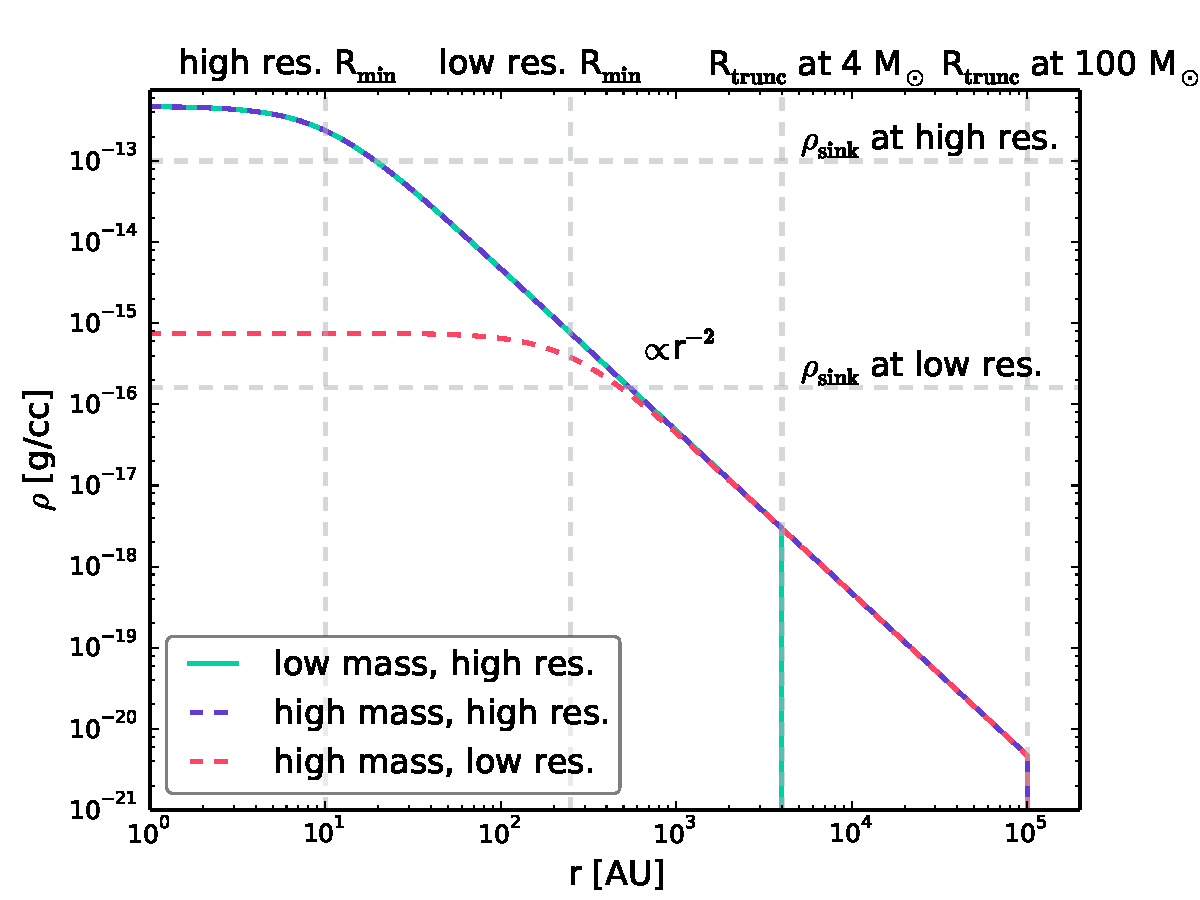
\includegraphics[width=0.85\textwidth]{Figures/new_nsis}
 \captionsetup{justification=justified,singlelinecheck=false,width=\linewidth}
 \decoRule
 \caption[Singular isothermal sphere profile]{The singular isothermal sphere profiles: The turquoise line shows the particular singular isothermal sphere profile of the low mass setup.
                                              The dashed lines in blue/red show the initial conditions for high mass spheres of 100 M$_{\odot}$.
                                              Radius parameters R$_{min}$ limit the central core densities and adjust the maximal resolutions of the collapse simulations.
                                              They were set to 10 AU for high resolution and 250 AU for low resolution.
                                              Truncation radii $R_{trunc}$ were set to 4000 AU and 0.485 pc, for low and high mass spheres respectively.}
\label{fig:nsis}
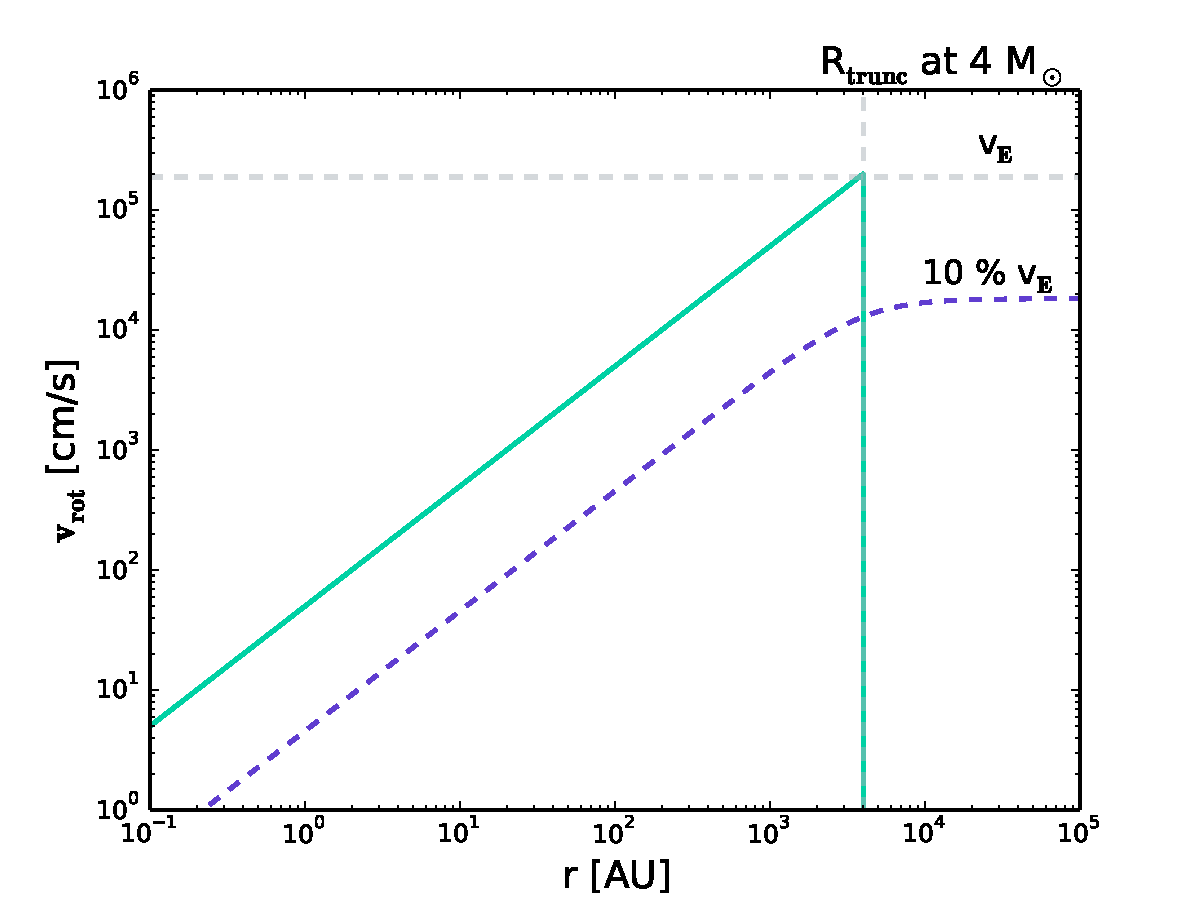
\includegraphics[width=0.85\textwidth]{Figures/solid_rot}
\captionsetup{justification=justified,singlelinecheck=false,width=\linewidth}
\decoRule
\caption[Rotational velocity profile]{The rotational velocity profiles: This plot shows the absolute of rotation velocities in the z=0--plane.
                                      Such a profile was used for all the runs with a mass of $4\,M_{\odot}$ and a truncated radius of $R_{trunc}=4000\,\text{AU}$.
                                      $v_{E}$ is the escape velocity, which is the minimal velocity an object needs to break free of the gravitational potential of the orbited central body.
                                      Later on, when the high--mass isothermal sphere collapses were investigated, these rotation profiles had to be changed for bigger spheres in order to avoid unrealistically high velocities.
                                      The velocity profiles were therefore smoothly connected to a value of 10 \% of the escape velocity and kept constant throughout the rest of the spheres.}
\label{fig:rot_vel}
\end{figure}
\FloatBarrier


%\newpage
% Reference runs ----------------------------------------------------------------------------------------
\section{Reference runs}
\label{sec:Reference_runs}

Pure--hydrodynamical simulations build a base line, to which the simulations including radiative transfer can be compared.
For all such simulations a polytropic equation of state was implemented; see \figref{fig:isotropic_hack}.
Of course, this equation of state is inspired by the behavior expected in star formation.
This allows the simulations to mimic the formation of the first Larson core where the medium becomes optically thick to radiation and consequently heats up without actually including radiative transfer.
In the low--resolution simulations however, the sink density threshold had to be lowered to account for the low resolution, which made them effectively isothermal.
For those runs that could resolve the Jeans length at the opacity limit, the temperature climbed to maximally 16 K.

Since this method is based on an idealized model, the first phase during the collapse maintains a very symmetric fragmentation pattern of which the \code{scaled\_up\_isoknee\_sink} run shows a nice example in \figref{fig:isotropic_binaries}.
Although some of the simulations produced expected behavior such as very symmetric binary--like fragmentation patterns, this indirect method of modeling star formation is not realistic.

Other reference simulations have been also performed and can be found in the same Table \ref{tab:hydro_pure}, all with \code{rt=.false.}
Some of them were evolved for so long that the rotating disk is totally destroyed by fragmentation.

The disks in purely--hydrodynamical simulations start to fragment due to the fact that without radiation the gas cannot reach high enough temperatures to prevent fragmentation and there are no steady, opposing forces to keep gravity at bay.
Thus, the results are very high sink particle numbers with low masses on average.
After around 100 kyrs, all pure--hydrodynamical simulations have converted at least 50\% of gas mass into sinks.

\begin{figure}[!htb]
 \centering
 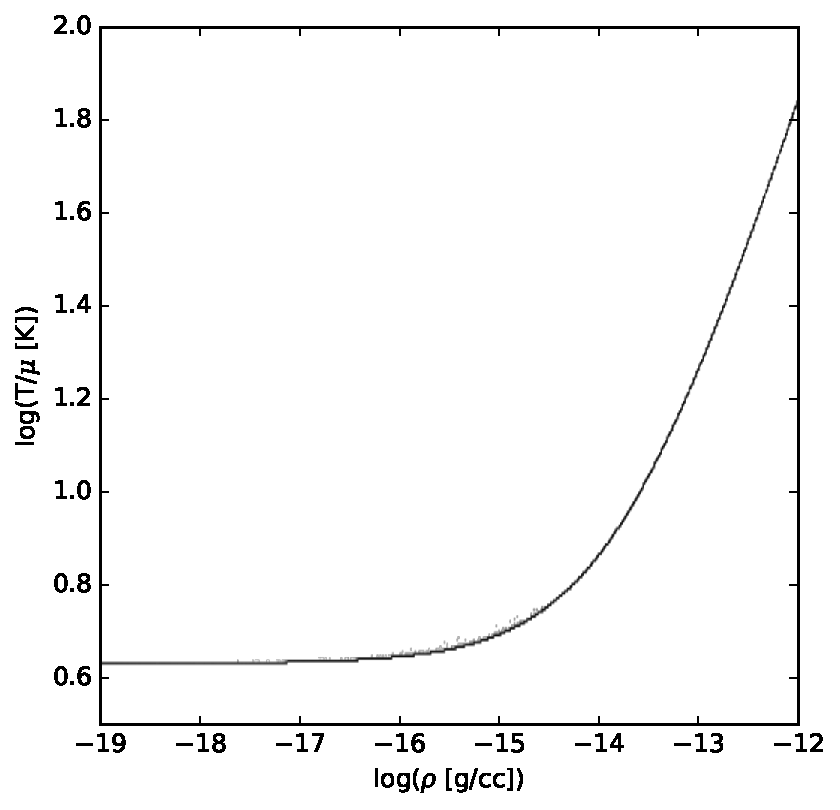
\includegraphics[width=0.8\textwidth]{Figures/isotropic_hack}
 \captionsetup{justification=justified,singlelinecheck=false,width=\linewidth}
 \decoRule
 \caption[Polytropic EOS]{The density--temperature phase plot of run \code{scaled\_up\_isoknee\_sink} at around 10.4 kyrs.
                          At the knee density of $10^{-14}$ g/cc the temperature increases quasi--adiabatically.
                          The EOS is the same for all purely--hydrodynamical runs.
                          It presents a poor--mans version of radiative transfer as it imitates the formation of the first Larson core at the opacity limit without actually performing radiative transfer.}
\label{fig:isotropic_hack}
\end{figure}
\FloatBarrier

\begin{figure}[!htb]
 \centering
 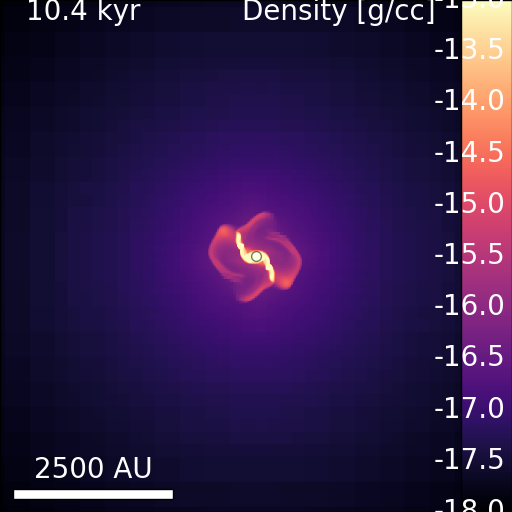
\includegraphics[width=0.6\textwidth]{Figures/isotropic_binaries}
 \captionsetup{justification=justified,singlelinecheck=false,width=\linewidth}
 \decoRule
 \caption[Fragmentation pattern]{A single snapshot of run \code{scaled\_up\_isoknee\_sink} which is a high--resolution, high--mass run.
                                 The symmetrical fragmentation patter is similar to those observed by \citet{Commercon_binaries}.
                                 This confirms the purely--hydrodynamical simulations and validates their use in comparison with radiation hydrodynamics simulations later.}
\label{fig:isotropic_binaries}
\end{figure}
\FloatBarrier

The reference runs also show another interesting feature which was already predicted in \secref{subsec:Instabilities}.
The self--similarity of the profile of a singular isothermal sphere implies that free--fall of matter towards the center is always steady.
\figref{fig:smaccm_selfsim} shows only one of many confirmations that isothermally collapsing cores are accreting with a constant rate of $\dot{M}_{acc} \sim \frac{c_{s}^{3}}{G}$.
During the whole simulation, the accretion rate seems to be fairly steady until most of the gas has been consumed and the sink reaches a maximal mass.

\begin{figure}[!htb]
 \centering
 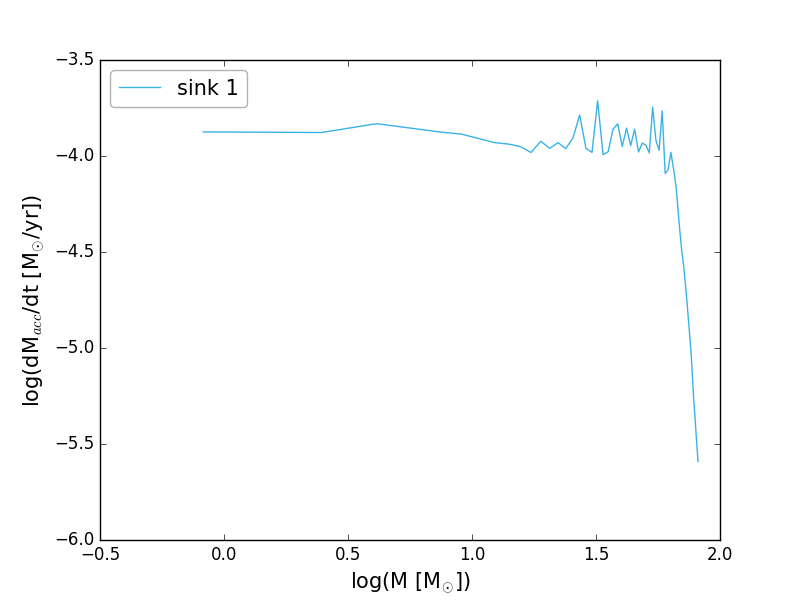
\includegraphics[width=0.75\textwidth]{Figures/smacc_m_selfsim_merge}
 \captionsetup{justification=justified,singlelinecheck=false,width=\linewidth}
 \decoRule
 \caption[Sink accretion rate plot of a pure--hydrodynamics run]{Accretion rate plot of the most massive sink formed in the high--mass low--resolution simulation \code{self\_similar\_iso\_merge}.
                                                                 Due to the isothermal sphere collapse, the accretion rate is steady at around $10^{-4}$ M$_{\odot}$ per year.
                                                                 Once most of the gas mass is consumed, the sink mass settles at a final value.}
\label{fig:smaccm_selfsim}
\end{figure}
\FloatBarrier

%\newpage
% Core collapse simulations - Comparison of HD with RHD ----------------------------------------------------------------------------------------
\section{Disk fragmentation}
\label{sec:Idealized_core_collapses}

For all variants of initial conditions (low--mass high--resolution, high--mass high--resolution, and high--mass low--resolution simulations) pure--hydrodynamics as well as radiation hydrodynamics simulations have been conducted.

\figref{fig:hydro_purePt2} shows snapshots of such a reference simulation, in which the low--mass, high--resolution initial conditions were used.
The excessive fragmentation can clearly be seen in the second panel on the left side.
Further details can be found in the overview in Appendix~\ref{sec:Overview} in Table \ref{tab:hydro_pure} under \code{ref\_run}.

In \figref{fig:rhd_snapshots} the same simulation with radiation can be seen.
The differences of both are enormous.
While in the reference run the disk already totally fragmented after 20 kyrs and formed many low mass sink particles, the simulation with radiation formed only one massive sink in the center of a fairly stable disk.

The need for radiation hydrodynamics is not just evident by this problem mentioned above.
Fragmentation of isothermal, hydrodynamical collapse simulations is excessive and produces too many sink particles.
To show and analyze the difference between pure--hydrodynamics and radiation hydrodynamics simulations, we introduce the \textit{Toomre parameter}

\begin{equation}
  Q = \frac{\omega c_{s}}{\pi G\Sigma}
\end{equation}

where $\omega$ is the epicyclic frequency of the central sink, $c_{s}$ the local sound speed in the gas and $\Sigma$ the surface density of the disk.
The Toomre criterion states that for $Q>1$ the disk can be considered stable against further collapse, whereas for $Q<1$ it is unstable.

It combines the parameter to express the balance between radiation, rotation and gravity.
The parameter $\omega$ describes the orbital frequency of the sink produced by rotation.
The greater the rotational velocity is, the more stable the disk is against gravitational collapse.
If $\omega$ increases, so does the Toomre parameter.
Radiation is another component opposing gravity.
$c_{s}$ is proportional to the temperature of the gas.
Accordingly, if the disk heats up and increases $c_{s}$ due to either internal friction or radiation, $Q$ increases.
The surface density term $G\Sigma$ incorporates the gravitational strength and tendency of the disk to collapse.

The criterion also indirectly represents a trend of the disk to regulate and stabilize itself.
If $Q<1$, the gravitational collapse proceeds and $\Sigma$ increases.
However, in this case there is more mass for the sink to accrete in the center.
Since the radiation emitted at the sink, the accretion luminosity, is proportional to the mass, the radiation subsequently increases also.
The parameter $c_{s}$ therefore increases and works towards the stabilization of the disk.

The Toomre parameter analysis for the collapsed disks of the low--resolution and high--resolution simulations reveals interesting properties.
\figfigref{fig:Toomre_hydro}{fig:Toomre_rt} show Toomre profiles of two runs with the mere difference that one of them is purely--hydrodynamical (not radiative transfer, simply a polytropic EOS), while the other involves radiative transfer.
In the comparison of both, it can be seen that the run with radiative transfer is more stable, especially in the range of radii for which the pure--hydrodynamical simulations tend to be unstable.
In fact, this is a trend detectable with all self--similar and scaled--up runs for which a pure--hydrodynamical and radiative transfer version was performed.
In the region where the central sink heats up the gas by irradiating it in the infrared spectrum, the Toomre parameter is raised and therefore the disk around the sink tends to be more stable.

This is also recognizable in the direct snapshots of the simulations in \figfigref{fig:hydro_purePt2}{fig:rhd_snapshots}, each on the left side of the second panel.
There, the influence of radiation can be observed through the gas' appearance.
Though radiation the gas' temperature rises, appears therefore more diffuse, and does not collapse to filaments and clumps at all or not as fast as in pure--hydrodynamics simulations.

\begin{figure}[!htb]
 \centering
 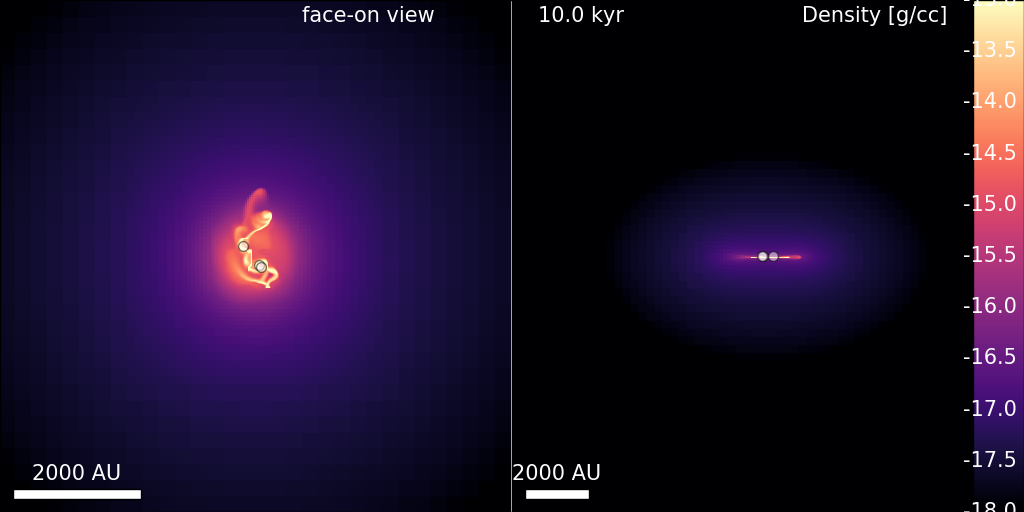
\includegraphics[width=0.95\textwidth]{Figures/hydro_pure/pure_hydro_1}
 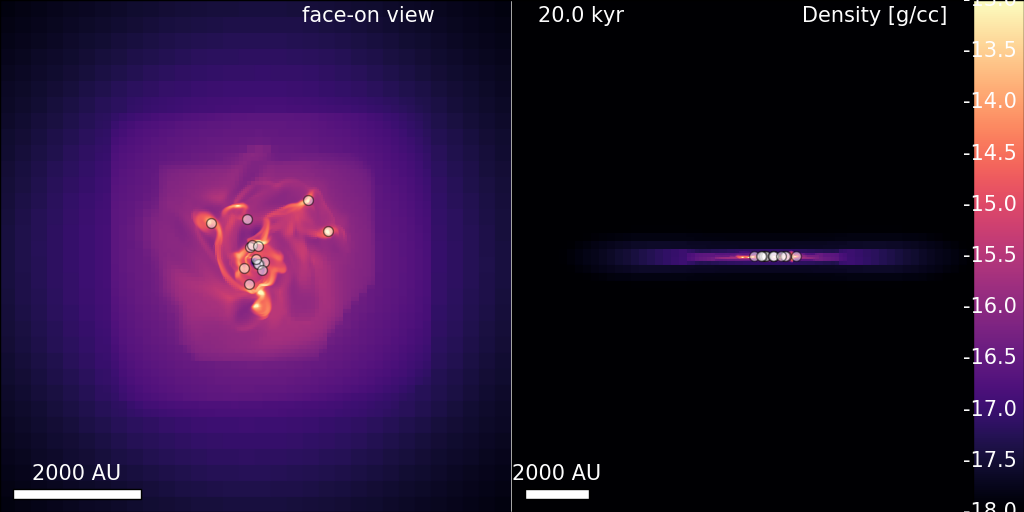
\includegraphics[width=0.95\textwidth]{Figures/hydro_pure/pure_hydro_2}
 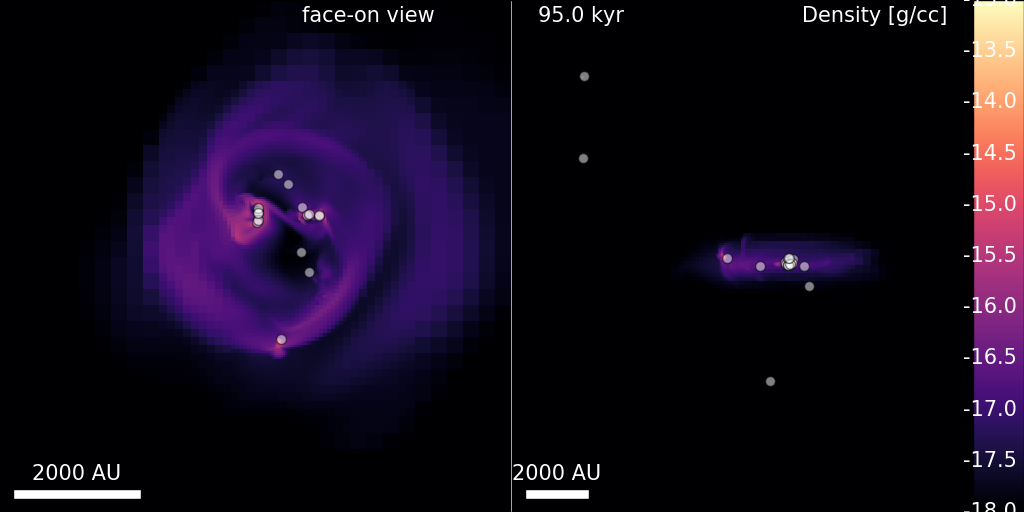
\includegraphics[width=0.95\textwidth]{Figures/hydro_pure/pure_hydro_3}
 \captionsetup{justification=justified,singlelinecheck=false,width=\linewidth}
 \decoRule
 \caption[Hydrodynamical isothermal sphere collapse]{Snapshots of a high--resolution, low--mass pure--hydrodynamics reference run \code{ref\_run}.
                                                     Its initial conditions correspond to a rotating singular isothermal sphere profile as described in \secref{subsec:Initial_conditions}.
                                                     The right side of each panel shows the formation of a disk due to the angular momentum of the gas while falling onto the sink which was formed in the beginning.
                                                     Fragmentation sets in almost immediately after the formation of the first sink as there are no opposing forces against gravity.
                                                     The result is a very turbulent disk with a high sink formation rate.}
\label{fig:hydro_purePt2}
\end{figure}
\FloatBarrier

\begin{figure}[!htb]
 \centering
 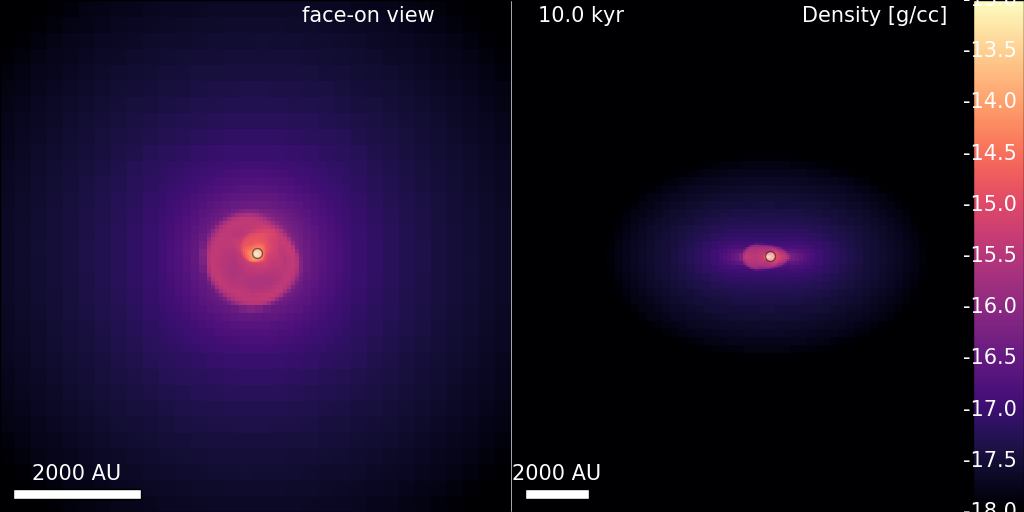
\includegraphics[width=0.95\textwidth]{Figures/rhd/multi_00039}
 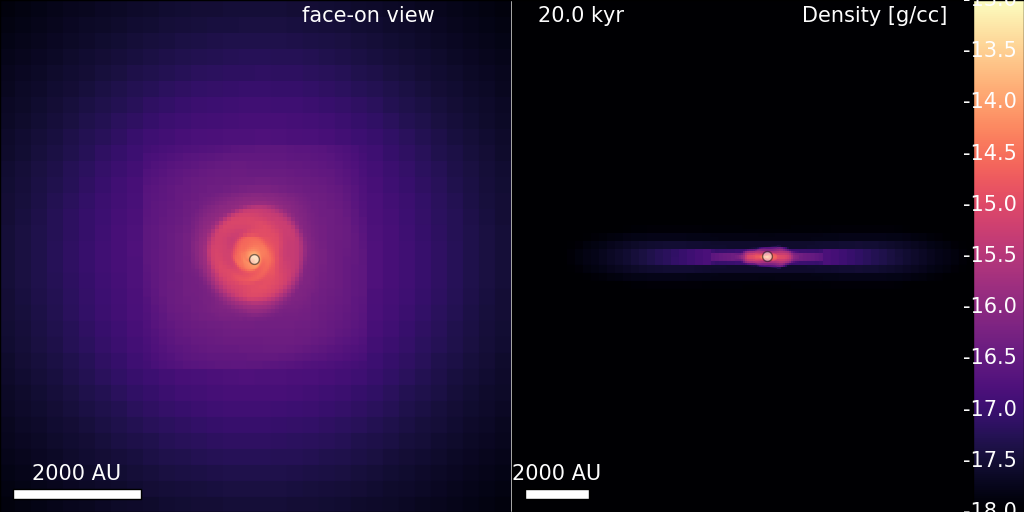
\includegraphics[width=0.95\textwidth]{Figures/rhd/multi_00079}
 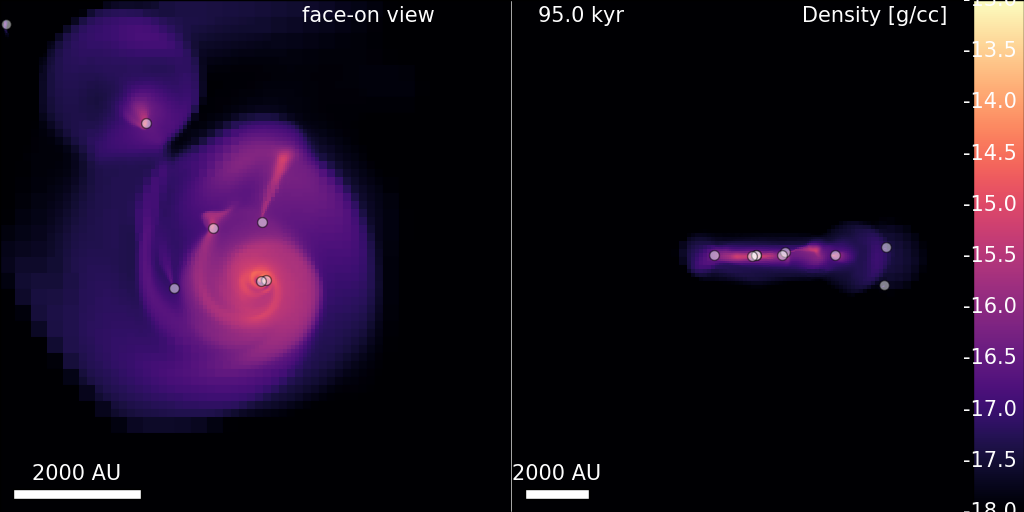
\includegraphics[width=0.95\textwidth]{Figures/rhd/multi_00379}
 \captionsetup{justification=justified,singlelinecheck=false,width=\linewidth}
 \decoRule
 \caption[Radiation hydrodynamical sphere collapse]{Snapshots of a high--resolution, low--mass radiation hydrodynamics run \code{nsub\_const\_rtc}.
                                                    This run's only difference to the one in \figref{fig:hydro_purePt2} is that radiative transfer is included.
                                                    In comparison of both, we see that here the resulting disk is thicker and its gas smoother due to the heat induced by the infrared radiation from the central sink.
                                                    Fragmentation only happens far from the central sink where the radiation has not heated the gas.
                                                    These fragments form sinks and return to the center due to dynamical friction and the gravitational attraction of the central sink.
                                                    This is easily noticeable in the last panel as wakes tracing the sinks' paths.}
\label{fig:rhd_snapshots}
\end{figure}
\FloatBarrier


\begin{figure}[!htb]
 \centering
 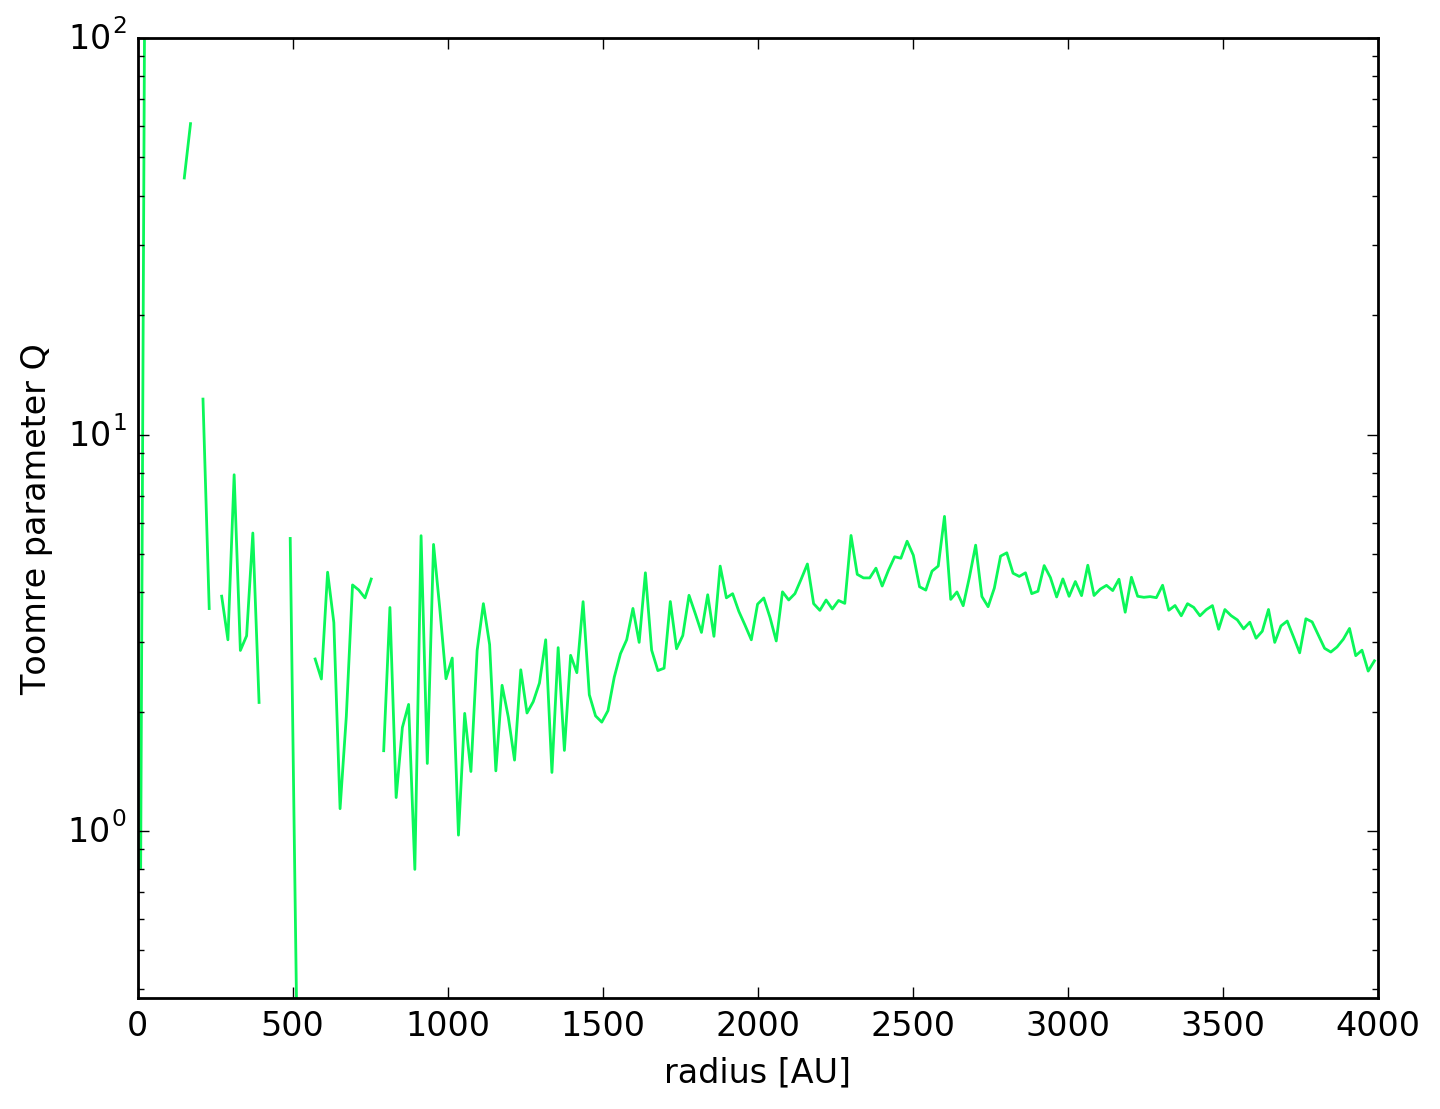
\includegraphics[width=0.85\textwidth]{Figures/toomre_hydro}
 \captionsetup{justification=justified,singlelinecheck=false,width=\linewidth}
 \decoRule
 \caption[Toomre profile of a pure--hydrodynamics run]{A Toomre profile of run \code{self\_similar\_iso\_merge}, a high--mass low--resolution simulation at a time of 1.24 Myrs, centered around the most massive sink.
                                                       It is a purely--hydrodynamical simulation, which showed a high degree of fragmentation.
                                                       It shows a tendency of gravitational instability around the radii between 500 and 1000 AU.}
\label{fig:Toomre_hydro}
\end{figure}
\FloatBarrier

\begin{figure}[!htb]
 \centering
 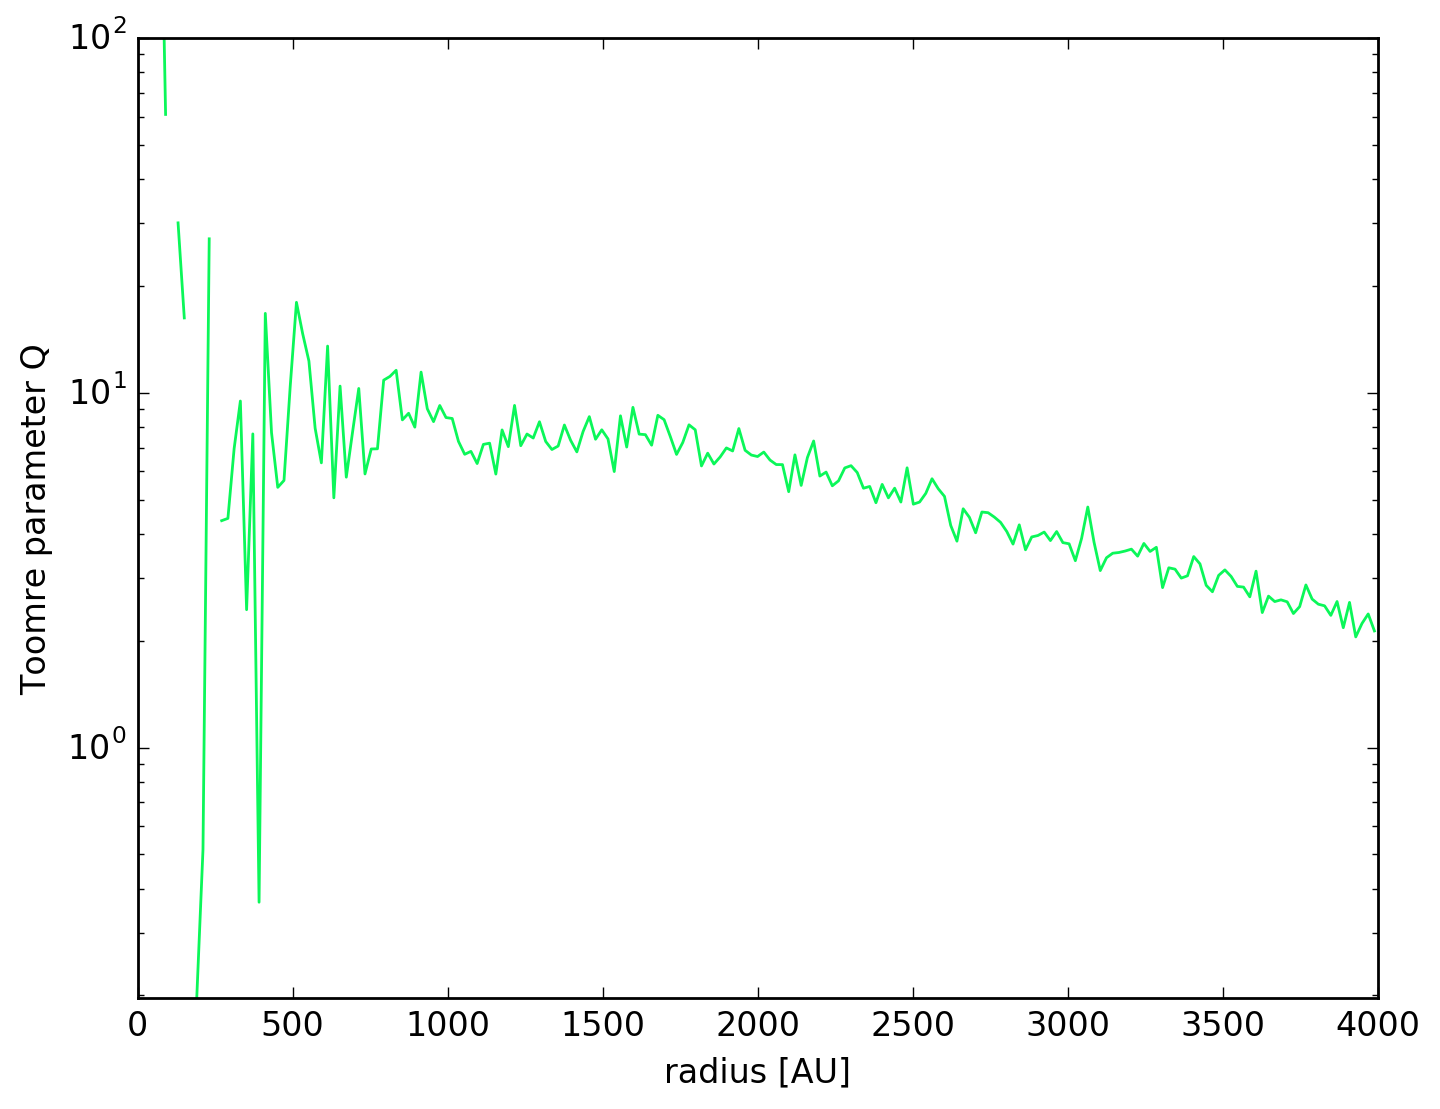
\includegraphics[width=0.85\textwidth]{Figures/toomre_rt}
 \captionsetup{justification=justified,singlelinecheck=false,width=\linewidth}
 \decoRule
 \caption[Toomre profile of a radiative transfer run]{A Toomre profile of run \code{self\_similar\_merge}, a high--mass low--resolution simulation at a time of 1.24 Myrs, centered around the most massive sink.
                                                      The same initial conditions were implemented as for the run in \figref{fig:Toomre_hydro} with the exception that this simulation included radiative transfer.
                                                      When compared to the previous \figref{fig:Toomre_hydro}, most of the values of $Q$ are clearly above 1, indicating gravitational stability.}
\label{fig:Toomre_rt}
\end{figure}
\FloatBarrier


%\newpage
% Cloud simulation----------------------------------------------------------------------------------------
\section{Molecular cloud}
\label{sec:MC}

Having thoroughly tested the numerical and physical influence of radiation onto an astrophysical fluid, the initial conditions for an entire molecular cloud simulation were prepared.

In the evaluation of the previous tests, especially of the runs' duration, it was deemed unnecessary to utilize the implementation of variable speed of light, since there is almost no speed--up, and in some cases it even prolonged the simulations.
However the subcycling of the RT routines seemed to provide a considerable gain in simulation speed without a grave loss in accuracy.
Again, only infrared radiation was used in the simulation.
Hence, the parameters of the radiative transfer module were calibrated such that the radiation travels at a constant fraction of the actual speed of light.

The RSL was calculated according to \citet{Skinner_Ostriker}.
They calculated the reduced speed of light depending on the maximum of the initial turbulent velocity dispersion $\sigma$, the sound speed $c_{s}$ and the optical depth of the initial uniform cloud $\tau$.

\begin{equation}
  \tilde{c} \geq (\sigma + c_{s})\mathrm{max}(\tau, 1) \qquad\quad \text{with} \quad \tau\equiv\frac{3}{2}\kappa_{P}\Sigma_{cloud}
\label{eq:Skinner_Ostriker_RSLA}
\end{equation}

where $\Sigma_{cloud}$ is the surface density of the initial cloud configuration determined by its mass M$_{cloud}$ and radius R$_{cloud}$.
The initial total gas mass of the cloud amounted to around M$_{cloud} \sim 2.4\times10^{4}$ M$_{\odot}$.
This mass was distributed in a spherical configuration with radius R$_{cloud} \sim 5$ pc.
The calculation of the optical depth for these parameters suggests that the global initial state of the cloud is quite far in the optically thin regime.
Therefore, the opacity limit $\tau = 1$ was applied in the approximation of the reduced speed of light.
The proportionality constant in the previous relation can be adjusted to the simulation.
In our case, a factor of 10 was used to stay on the more conservative side in the approximation.

Since highly turbulent gas flows are observed in almost all molecular clouds, they are a key component in such cloud simulations.
For this purpose, the sphere of mass M$_{cloud}$ and radius R$_{cloud}$ was actually carved out from another simulation and restarted.
In that simulation, the velocity field was driven by Gaussian random perturbations with a standard Kolmogorov power spectrum $E(k) \propto k^{-5/3}$.
Then, the simulation was run without self--gravity until nice groups of filaments formed, which roughly resemble actual observations of molecular clouds.
At that point, the relevant data within the sphere was saved in grafic--files, which can be read in by RAMSES as initial conditions.

The molecular cloud simulation took several weeks to complete, and even then it only progressed to around 1.5 Myrs.
Still, the simulation results reveal interesting properties.
Further information to some important parameters are listed below, in Table \ref{tab:cloud}.

\begin{table}[!htb]
\begin{adjustbox}{width=\textwidth}
\begin{tabular}{lccccccc}
\toprule
Name ID & rt & hydro\_only & isothermal & sink & scheme & riemann & slope\_limiter \\
\midrule
ir\_cloud & .true. & .false. & .false. & .true. & muscl & hllc & MinMod \\
\bottomrule
\toprule
\quad  & L [pc] & levelmin & levelmax & ncpu & time [Myr] & duration [h] & merging [kyr] \\
\midrule
\quad & 20 & 7 & 13 & 256 & 1.4921 & 384.42 & 5 \\
\bottomrule
\toprule
\quad & N$_{sinks}$ & M$_{tot}$ [M$_{\odot}$] & M$_{sink}$ [M$_{\odot}$] & RSL [km/s] & rt\_nsubcycle & $\kappa_{P}$ [cm$^{2}$/g] & $\kappa_{R}$ [cm$^{2}$/g] \\
\midrule
\quad & 104 & 12885.4389 & 1152.8 & 14.44 & 100 & 0.1 & 0.035 \\
\bottomrule
\end{tabular}
\end{adjustbox}
\captionsetup{justification=justified,singlelinecheck=false,width=\linewidth}
\caption[Cloud simulation parameter info]{Parameter information on the molecular cloud run at the end of the simulation.}
\label{tab:cloud}
\end{table}
\FloatBarrier

\figref{fig:CloudPt3} shows snapshots of the cloud simulation as it progresses.
Rather than displaying the radiation density, it was converted into radiation temperature $T_{rad}$ with
\begin{equation}
  T_{rad} = \Big(\frac{c n_{\gamma} \langle \epsilon \rangle}{c a}\Big)^{1/4}
\end{equation}

where $n_{\gamma}$ is the stored photon number density data, $\epsilon$ the average energy of the particular photon group, $a$ the radiation constant, and $c$ the speed of light.
This makes the radiation temperature comparable to the gas temperature.


\newpage
\thispagestyle{empty}
\begin{figure*}[!htb]
 \centering
 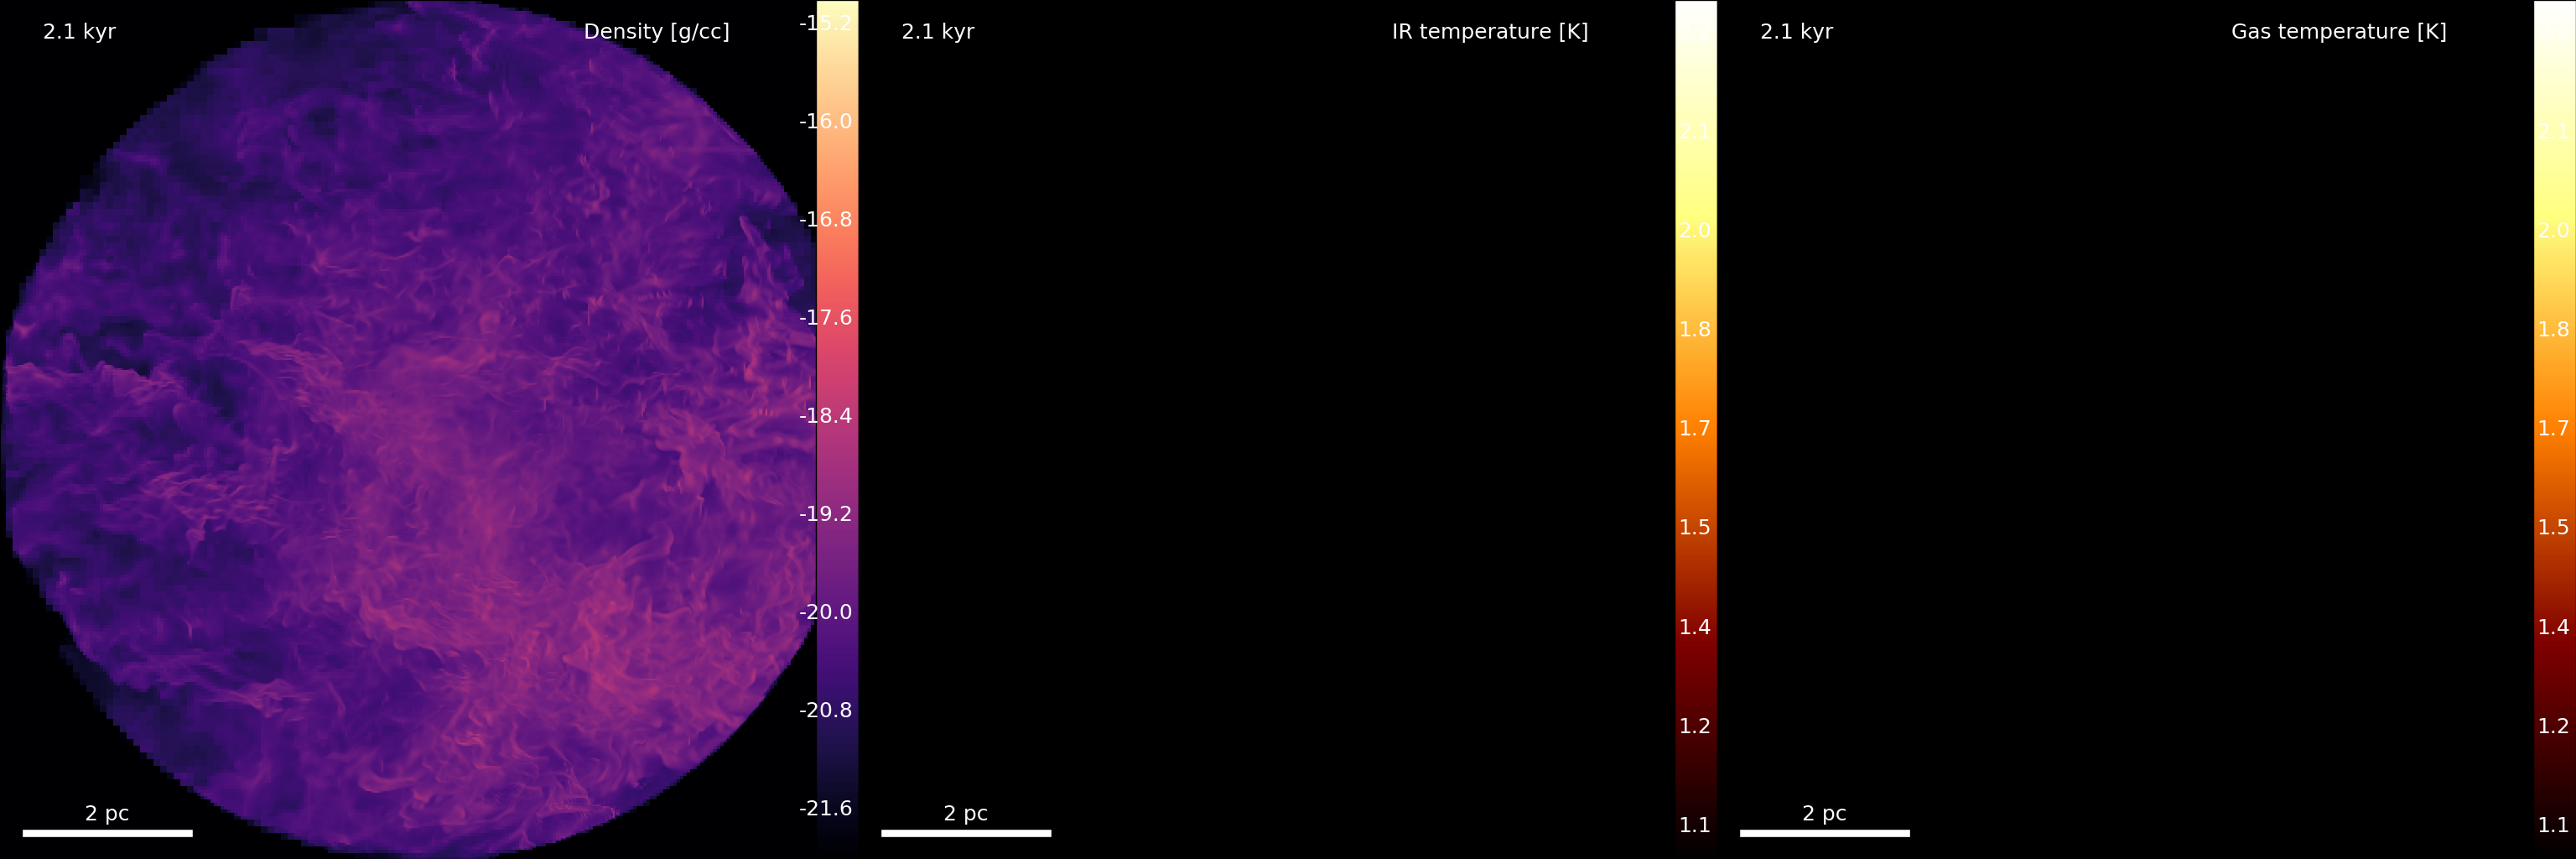
\includegraphics[width=1.05\textwidth]{Figures/cloud_snapshots/multi_00000}
 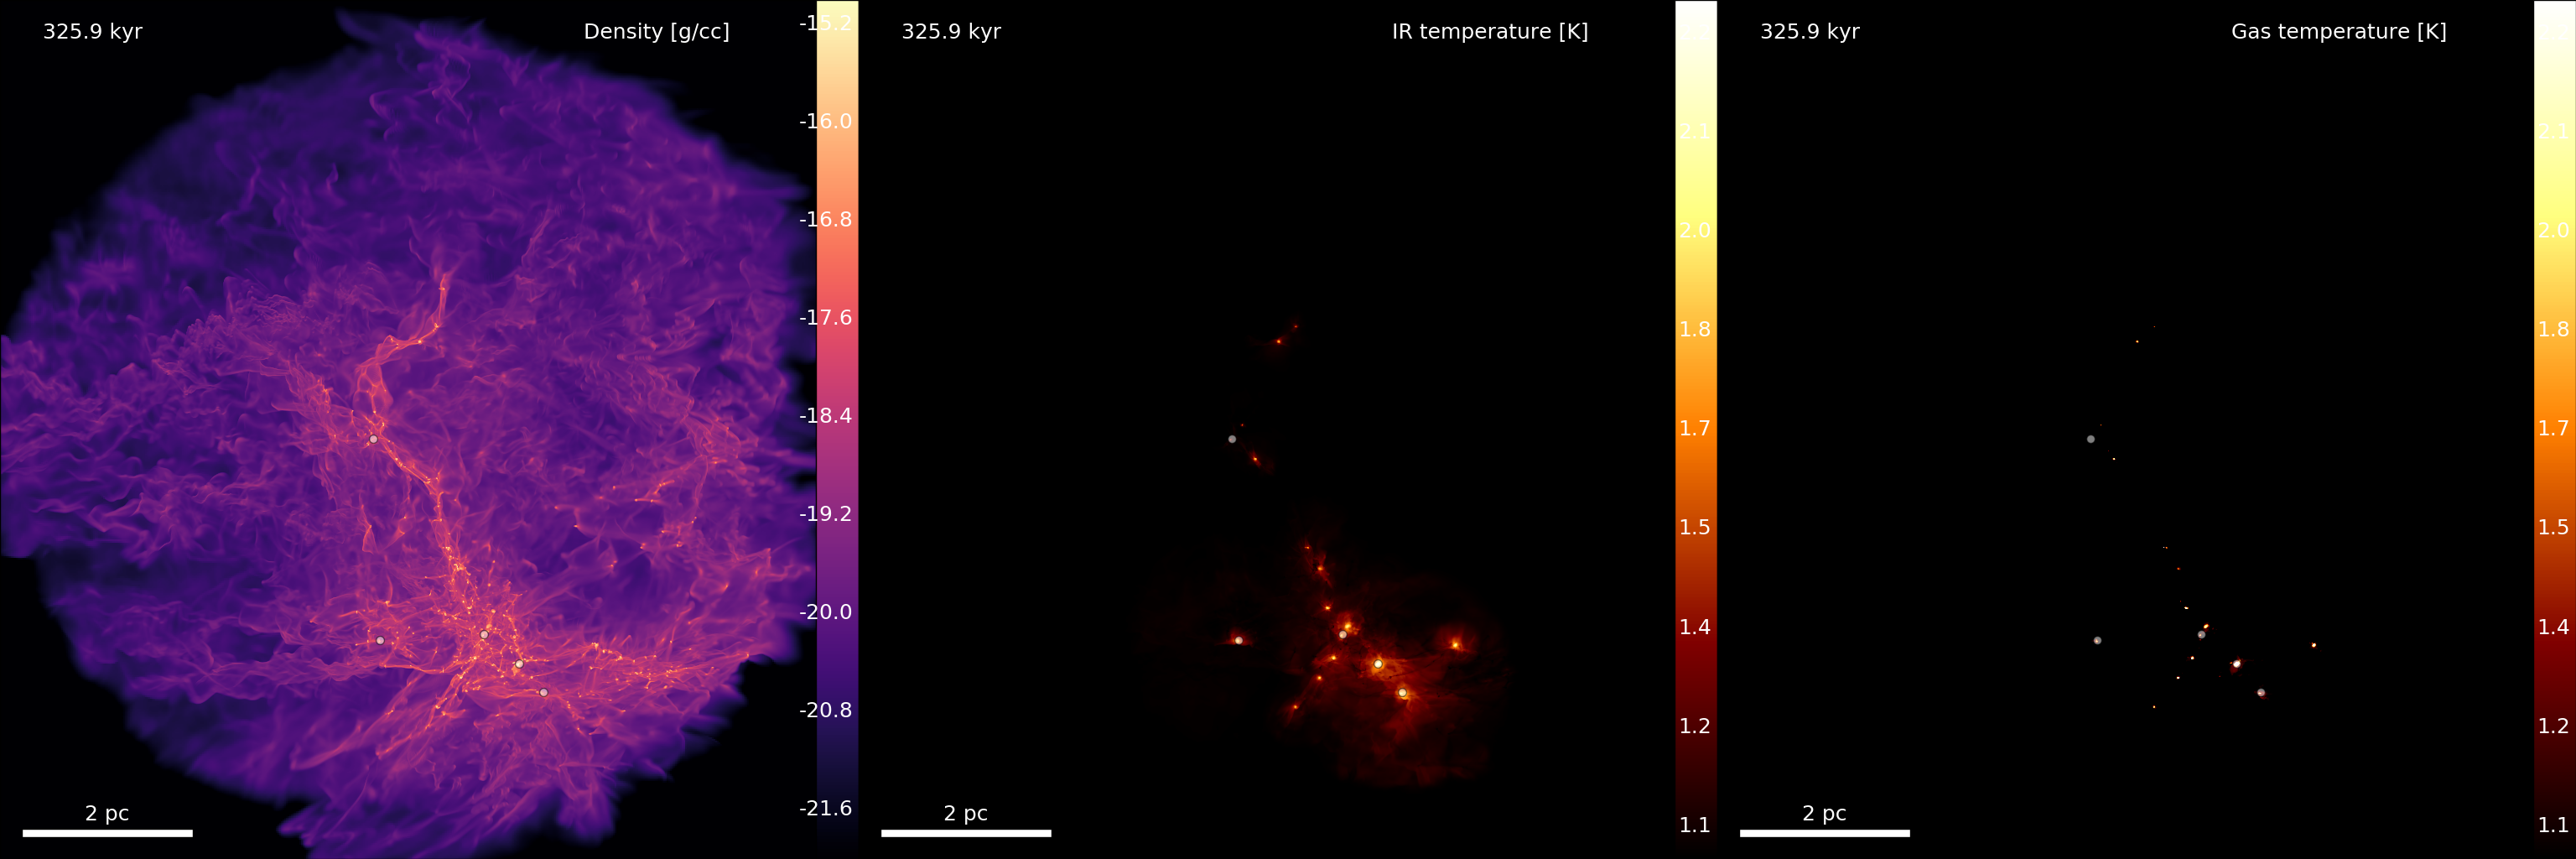
\includegraphics[width=1.05\textwidth]{Figures/cloud_snapshots/multi_00175}
 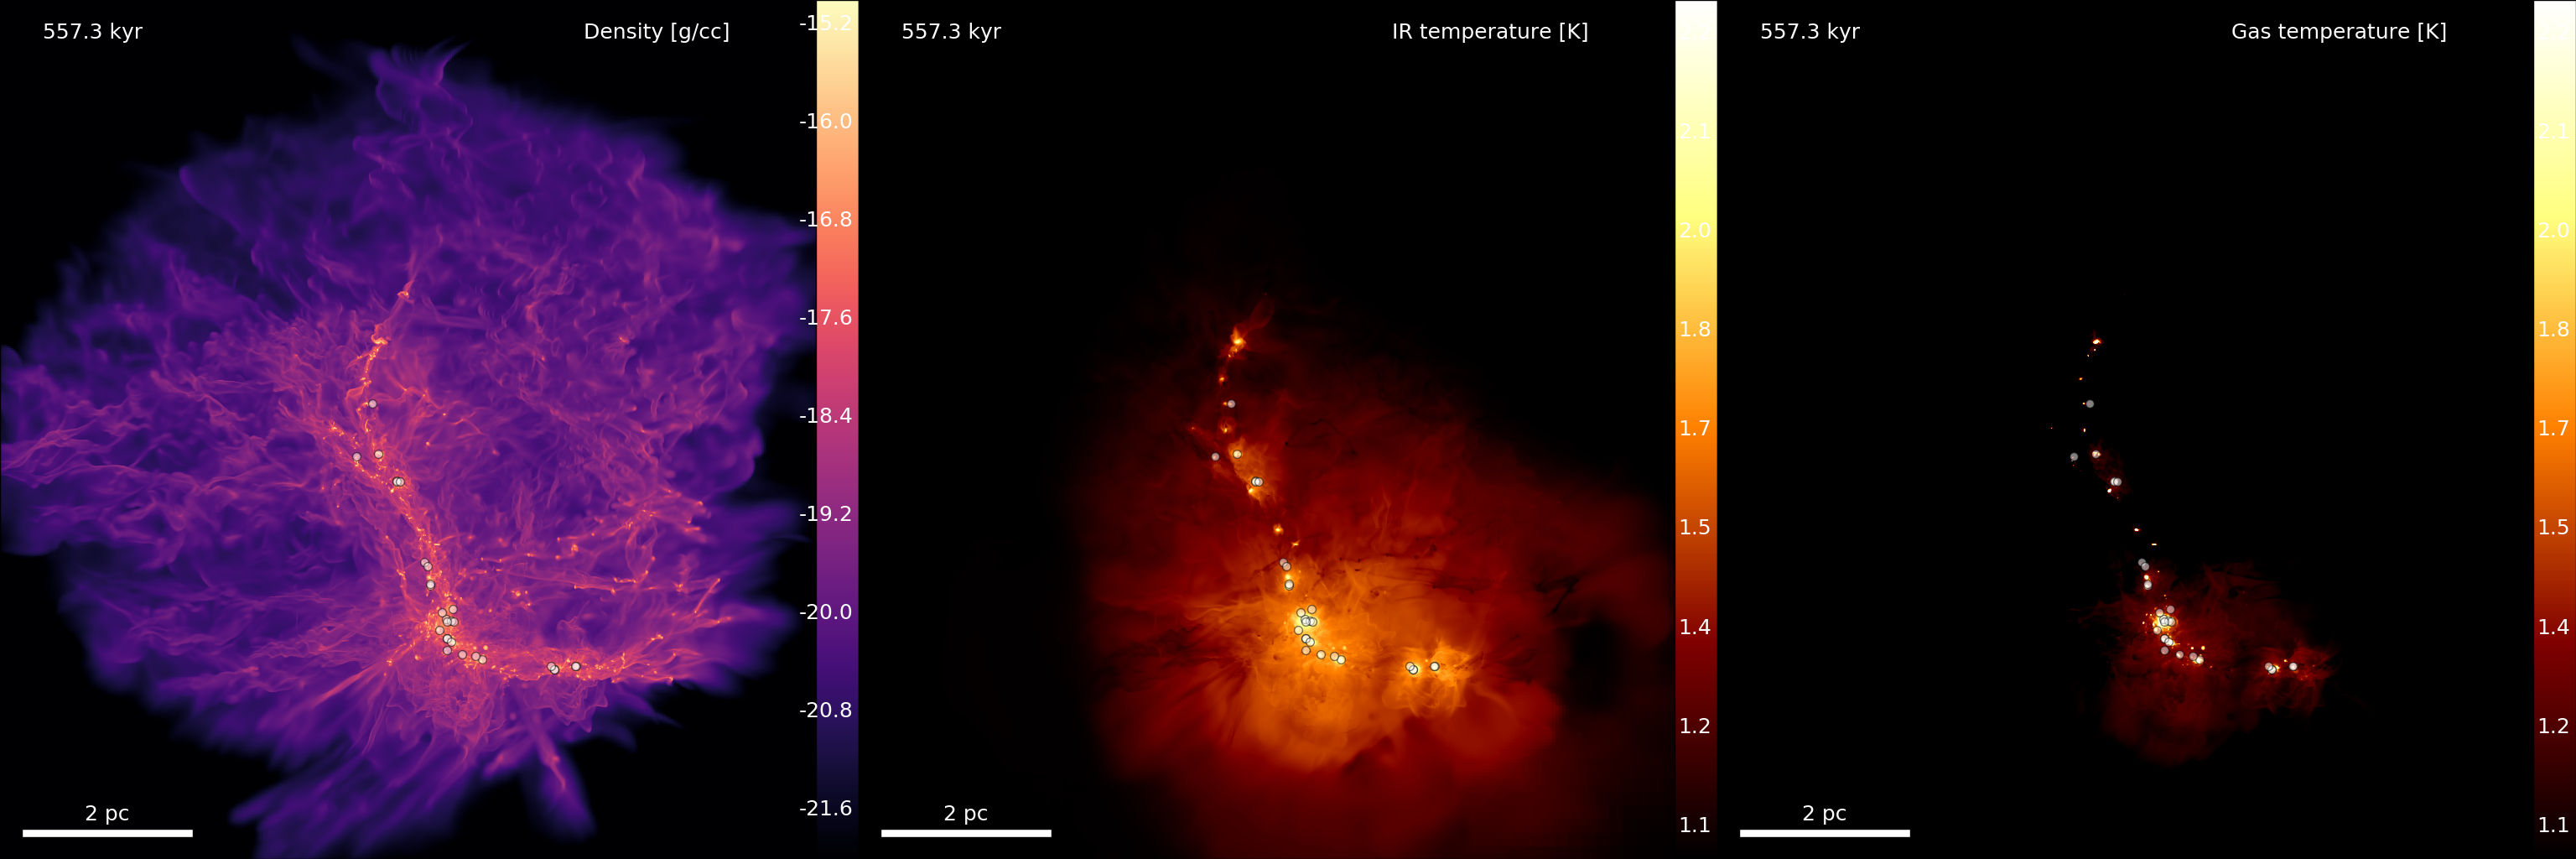
\includegraphics[width=1.05\textwidth]{Figures/cloud_snapshots/multi_00300}
 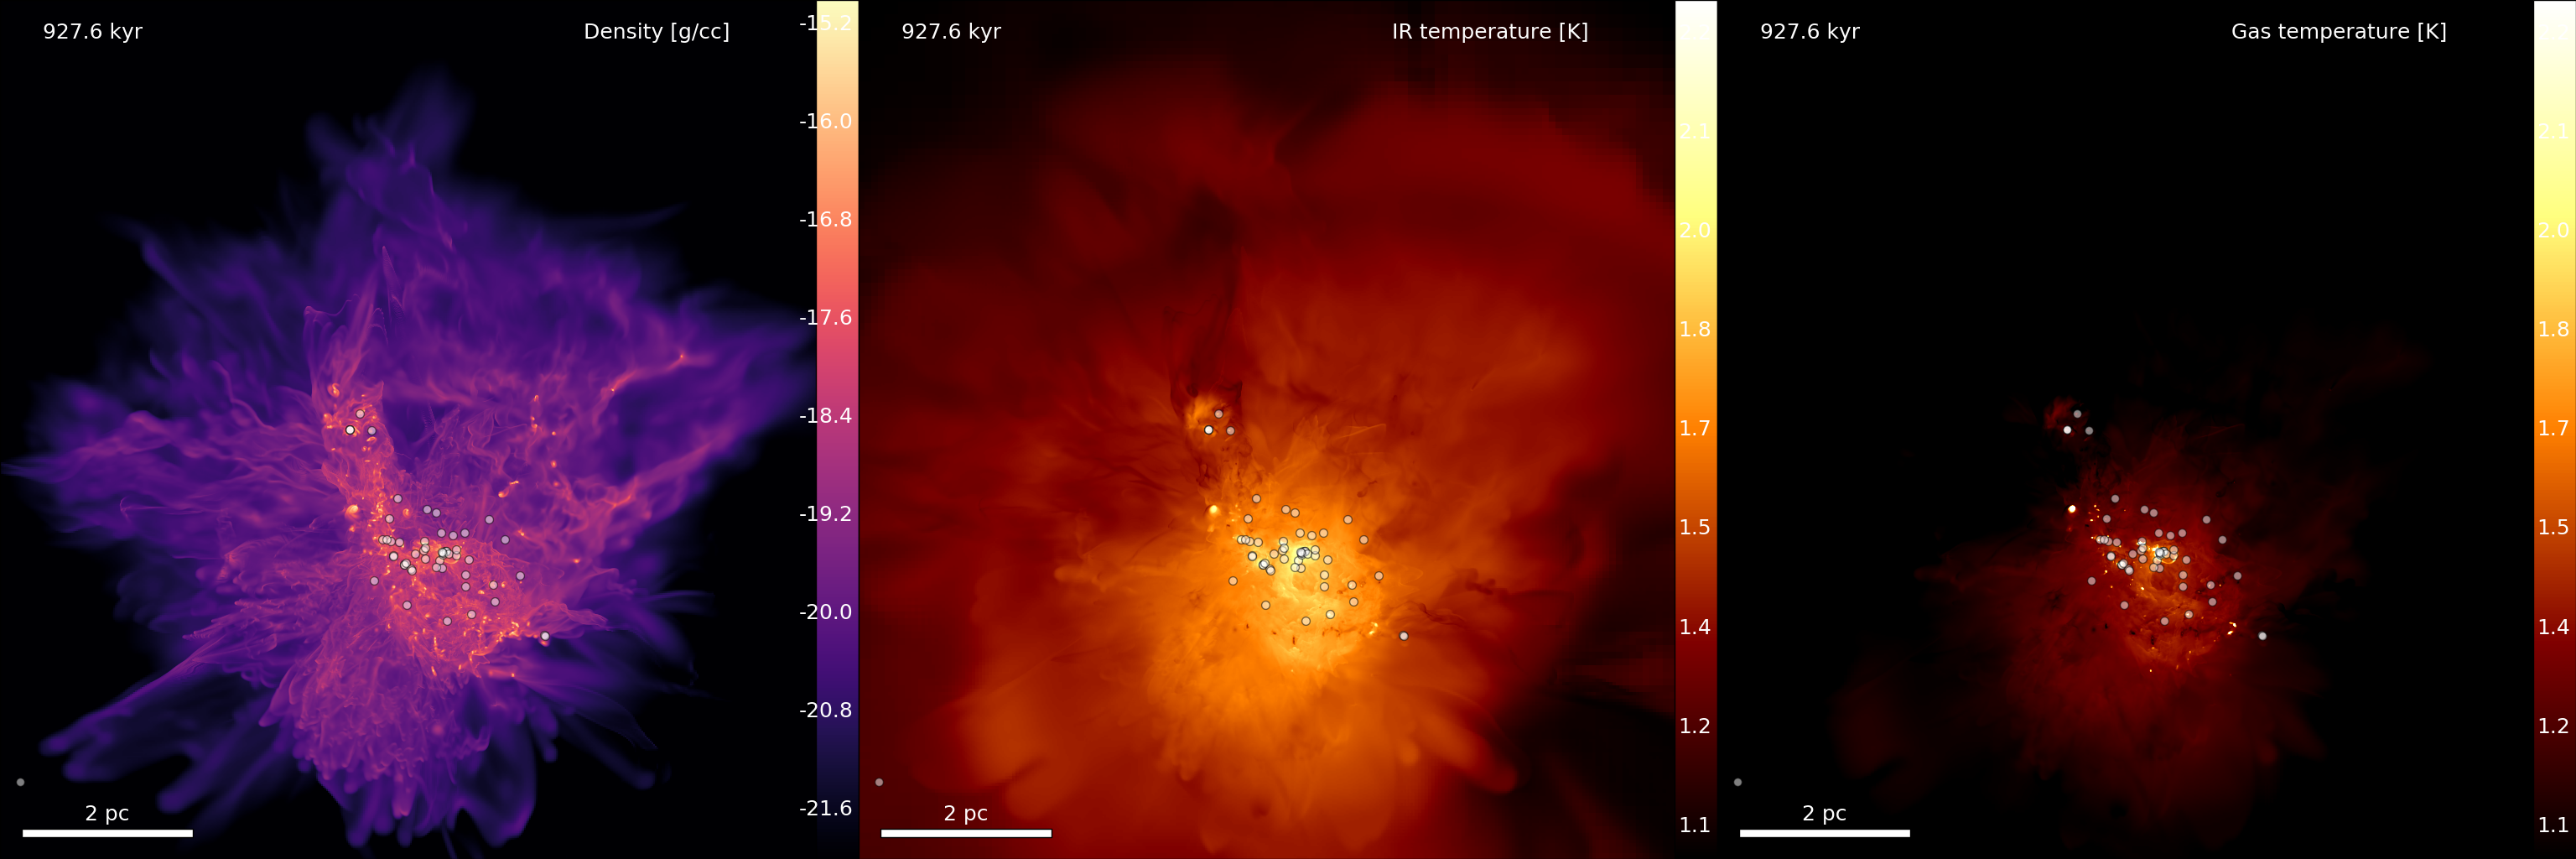
\includegraphics[width=1.05\textwidth]{Figures/cloud_snapshots/multi_00500}
 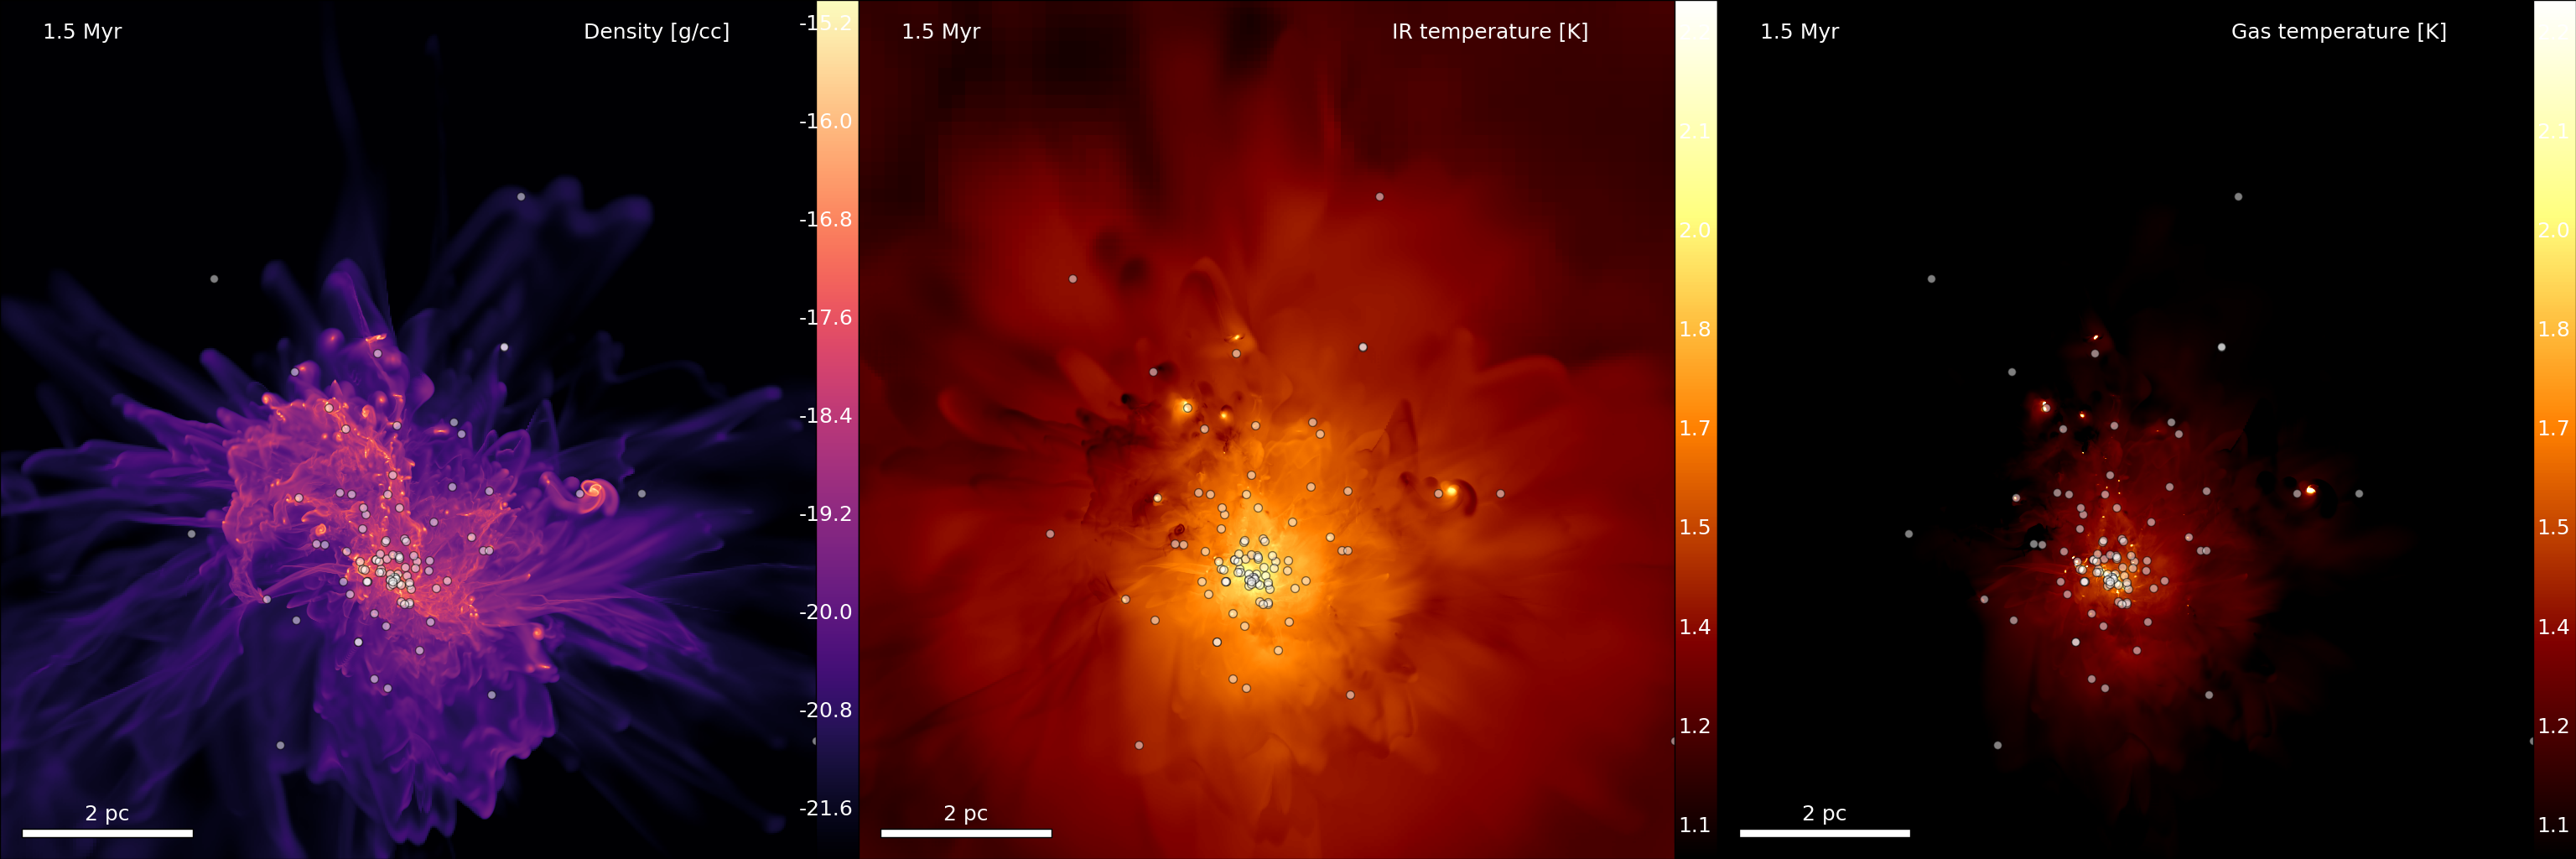
\includegraphics[width=1.05\textwidth]{Figures/cloud_snapshots/multi_00800}
 \captionsetup{justification=justified,singlelinecheck=false,width=\linewidth}
 \decoRule
 \caption[Molecular cloud simulation snapshots]{Snapshots of the molecular cloud's density, radiation and gas temperature.}
 \label{fig:CloudPt3}
\end{figure*}
\FloatBarrier


% Eddington ratio----------------------------------------------------------------------------------------
\subsection{Eddington analysis}
\label{subsec:Eddington_ratio}

\citet{Skinner_Ostriker} used in the analysis of their simulated cloud the Eddington ratio to quantify how strong radiation opposes gravity.
To follow their example we introduce the Eddington ratio

\begin{equation}
  f_{Edd}(r) = \frac{\kappa\rho F_{rad}}{c \rho g}
\label{eq:Eddington_ratio}
\end{equation}

where $\kappa$ is the frequency--averaged opacity, $F_{rad}$ the total radiation flux, and $g$ the gravitational acceleration towards the center.
It represents the fraction between radiational and gravitational force~\footnote{in this form, it actually describes a ratio of \textit{force densities}} exerted on the gas in the cloud.
Are the two forces in equilibrium the Eddington ratio is 1.
A value of the Eddington ratio $< 1$ indicates that the gas in the cloud feels a net inward force and vice versa.

In the simulation, sink particles act as radiation sources as a resulting effect of the mass accretion.
Therefore their luminosity $L_{rad}$ can be used as approximation for the radiation flux

\begin{equation}
  F_{rad} = \frac{L_{rad}}{4\pi r^{2}}
\end{equation}

This approximation unfortunately only holds further away from the sink in the optically thin regime.
For the optically thick regime, the diffusion limit has to be taken into account; see in \secref{subsec:Diffusion_limit}.

The diffusive limit with the assumption that gas and radiation are roughly in thermal equilibrium, fixes the flux in the optically thick regime.

\begin{equation}
  F_{rad} \simeq -\frac{c\lambda_{R}}{3} \nabla E \simeq - \frac{4ca}{3\kappa\rho} T^{3} \nabla T
\end{equation}

where $a$ is the radiation constant and $T$ the temperature of the gas.

The Eddington ratio as described by \eqnref{eq:Eddington_ratio} indicates the net force of two opposing forces, namely radiation and gravity.
Thereby, other influences have been neglected such as gas pressure gradients or centrifugal forces.

\begin{equation}
  \rho \frac{GM}{r^{2}} = \frac{4}{3}a T^{3}\nabla T + \rho \frac{k_{B} \nabla T}{\mu m_{H}} + \rho \frac{v_{\theta}^{2}}{r}
\end{equation}

Here, the left hand side describes the strong gravitational term, on the right hand side we have the radiation term, the gas pressure term, and the centrifugal term (in order).
Due to the temperature's high exponent in the radiation force term, radiation pressure gradients dominate over all other forces already at around 200 K for a gas at $10^{-15}$ g/cc.

This means that other force contribution might still play a role on the outskirts of the cloud, where the temperature is still very close to the modeled ISM temperature, but towards the center the radiation pressure dominates.

Figures~\ref{fig:Cloud_density}, \ref{fig:Cloud_temperature} and \ref{fig:Cloud_tau} show profiles of the cloud at a late time in the simulation.
At that time, already almost hundred sinks have formed and removed a considerable amount of gas mass from the cloud.
The center part of the cloud moved from an optically thin regime to a optical depth well beyond 1.
With the rise in sink number more and more radiation sources appeared.
The radiation emitted by them got trapped by the optically thick gas and heated the gas to the order of $\sim10^{2}$ K.

In combining these profiles according to \eqnref{eq:Eddington_ratio}, the Eddington ratio profile can be calculated; see \figref{fig:Cloud_eddington}.
It shows two Eddington ratio profiles, one with the flux approximated with the diffusion limit, the other with an optically thin flux approximation.
Their lines almost perfectly match, where the optical depth crosses the value 1.
The curves in their valid regimes are almost consistently below the Eddington limit, which indicates that a majority of the gas in the cloud still feels a net inward force.
This also agrees well with the findings of \citet{Skinner_Ostriker}.
However, the temperature of the cloud only started to rise towards $10^{2}$ K, which means other forces might still have some considerable influence on the gas.

\begin{figure}[!htb]
 \centering
 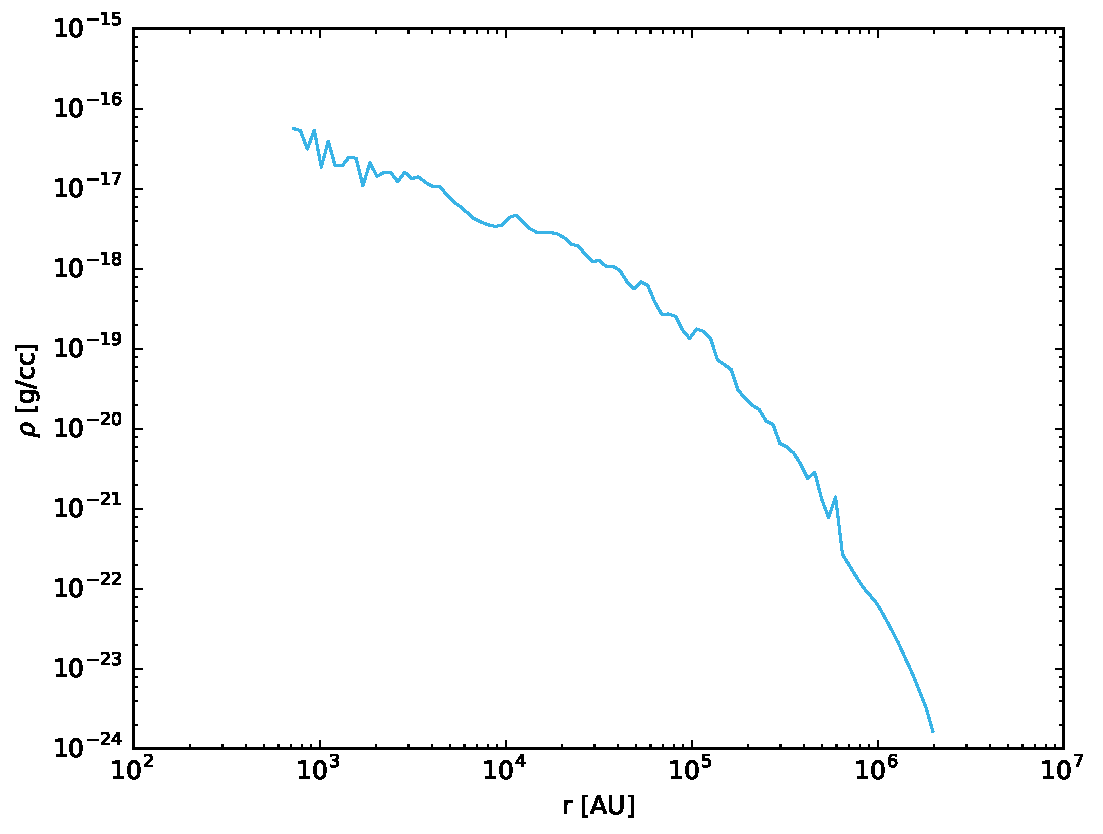
\includegraphics[width=0.9\textwidth]{Figures/cloud_profiles/density_profile}
 \captionsetup{justification=justified,singlelinecheck=false,width=\linewidth}
 \decoRule
 \caption[Cloud density profile]{The simulated cloud's density profile at a simulated time of 1.3724 Myrs.
                                 It includes the entire cloud's gas mass, but omits sink particle masses.}
 \label{fig:Cloud_density}
\end{figure}

\FloatBarrier

\begin{figure}[!htb]
 \centering
 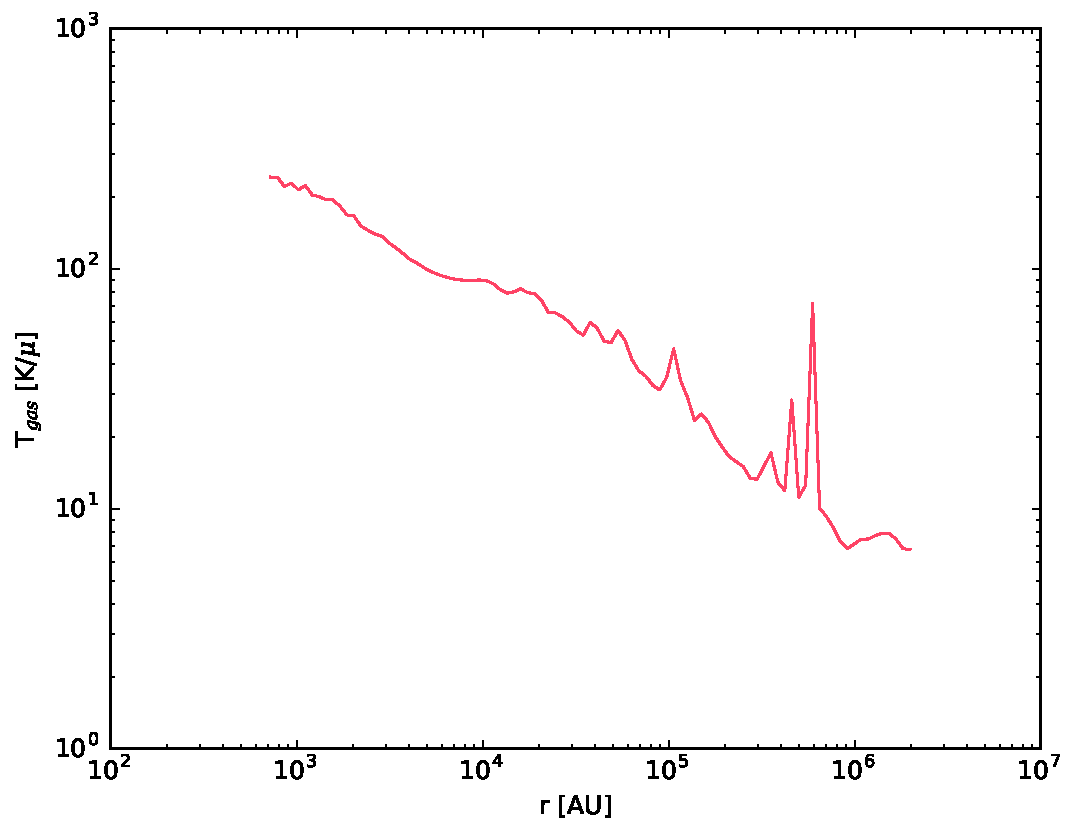
\includegraphics[width=0.9\textwidth]{Figures/cloud_profiles/temp_profile}
 \captionsetup{justification=justified,singlelinecheck=false,width=\linewidth}
 \decoRule
 \caption[Cloud temperature profile]{The simulated cloud's temperature profile at a simulated time of 1.3724 Myrs.
                                     Radiation emitted from sinks in the center of the cloud heat up the gas to almost 200 K.
                                     The peaks at $5\cdot10^{5}$ and $7\cdot10^{5}$ AU are due to very massive sinks with high luminosities heating the gas in their proximity.}
 \label{fig:Cloud_temperature}
\end{figure}

\FloatBarrier

\begin{figure}[!htb]
 \centering
 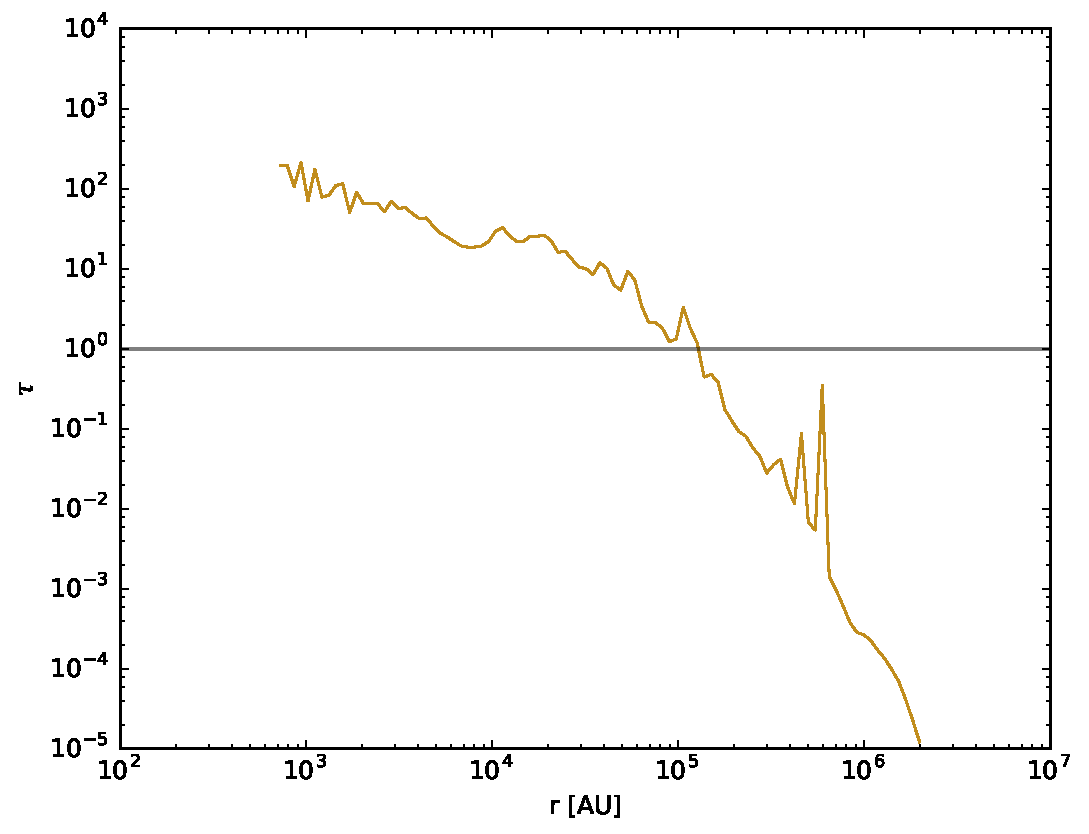
\includegraphics[width=0.9\textwidth]{Figures/cloud_profiles/tau_profile}
 \captionsetup{justification=justified,singlelinecheck=false,width=\linewidth}
 \decoRule
 \caption[Cloud's optical depth profile]{The simulated cloud's optical depth profile at a simulated time of 1.3724 Myrs.
                                         It is calculated according to \eqnref{eq:Skinner_Ostriker_RSLA}, with an opacity profile $\kappa\propto T^{2}$ according to \citet{Davisetal}.}
 \label{fig:Cloud_tau}
\end{figure}

\FloatBarrier

\begin{figure}[!htb]
 \centering
 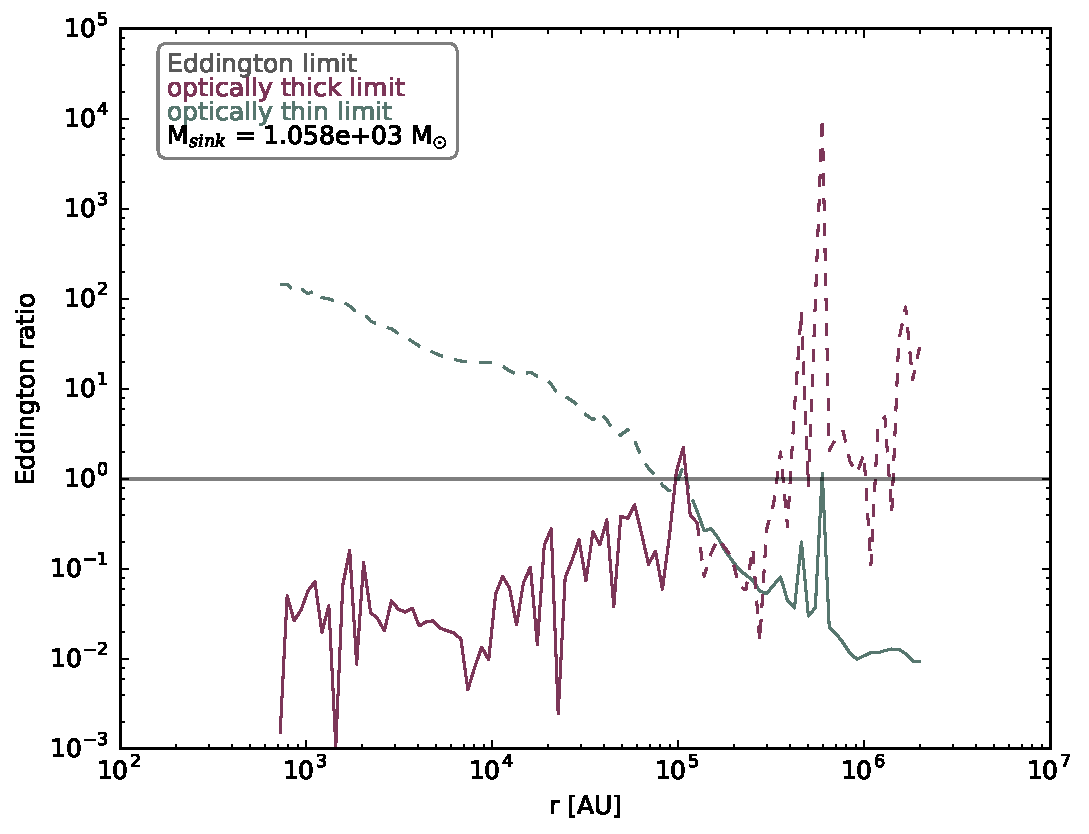
\includegraphics[width=0.9\textwidth]{Figures/cloud_profiles/eddington_limits}
 \captionsetup{justification=justified,singlelinecheck=false,width=\linewidth}
 \decoRule
 \caption[Cloud's Eddington ratio profile]{The simulated cloud's Eddington ratio profile at a simulated time of 1.3724 Myrs.
                                           Throughout the cloud the Eddington ratio lies below 1, indicating that a majority of the gas mass still feels the gravitational pull towards the center.}
 \label{fig:Cloud_eddington}
\end{figure}
\FloatBarrier


% Star cluster----------------------------------------------------------------------------------------
\subsection{Star cluster}
\label{subsec:Star_cluster}

The analysis of the star cluster in the center of the cloud reveals interesting circumstances.
At the end of the simulation, roughly half of the cloud's gas mass has been converted into sink particles.
The mass range of these particles goes from $\sim0.1$ M$_{\odot}$ up to $\sim1000$ M$_{\odot}$.
This range unfortunately does not conform with the initial stellar mass function described by \citet{Charbier, Kroupa}.
In the last snapshot of \figref{fig:CloudPt3} the most massive sink in the simulation can be seen leaving the cloud on the upper right.

The escape of the most massive sink from the cluster has grave consequences.
It throws the cluster off balance and de--virializes the system.
To understand the virialization of clusters, we introduce the virial parameter

\begin{equation}
  \alpha = \frac{2 E_{kin}}{E_{pot}} \sim \frac{2\cdot(1/2)M\sigma^{2}}{(3/5)GM^{2}R^{-1}} = \frac{5\sigma^{2}R}{3GM}
\end{equation}

where $\sigma$ is the cluster's velocity dispersion, $M$ the collective sink mass and $R$ the cluster's radius.

\figref{fig:Cluster_virial} presents the virial analysis of the simulation's cluster.
It shows what already was mentioned above.
The first panel describes the virial parameter of the cluster during the most critical time in the simulation.
At around 1 Myr a jump appears in the evolution of the virial parameter and disrupts the the cluster's equilibration.
This can be accredited to the escape of a massive sink, in fact the most massive in the simulation.
By leaving the cluster, it removes a considerable fraction of mass from the cluster.
Therefore, the virial parameter increases.
After a while the cluster tends to virialize again.
It is barely visible in the plot, however in the end of the simulation two medium sized sinks escape the cluster again which would increase the virial parameter again.
The second panel shows the rate with which the the gas is converted into sinks.
The rate is kept relatively steady and agrees well with the third panel.
It describes the similarly steady rate with which the sink particle number increases, or in a few cases decreases in which the sink particles merge.

The cloud simulation also shows some interesting differences to the reference run of the cloud with an polytropic EOS, we performed.
The pure--hydrodynamics reference run displays much higher sink numbers; see \figref{fig:Cluster_HDvirial}.
Gas to sink mass conversion percentages and relative sink count of the reference run are much higher in comparison, and the average sink mass is smaller by almost a factor of 6.
This also agrees with the findings of the idealized core collapses, where it was found that sink masses are much higher when radiation is included.
There the radiation slows down the collapse by heating the center region and thus supports the resulting disks, which enables the sinks to slowly form, accrete mass with a steady rate and consequently grow to a higher mass.
In the reference runs without radiation, the collapse is much faster, leading to fragmentation and therefore smaller sink masses.
Contrary to the reference run which shows no tendency to virialize, the star cluster of the RT--simulation tends to equilibrate.
It seems that the collapse of the cloud is 'quieter' and slower when radiation is involved, which enables the resulting star cluster to possibly equilibrate.
However, without radiation the collapse is much too fast and violent, which causes the emerging star cluster to explode.
This can also be seen in the beginning in the first panels of both figures.
Within 0.4 Myrs the star cluster from the reference run already reached the virial equilibrium line, whereas the star cluster with radiation
Nevertheless, based on the virial parameters at the end of both simulations alone, both clusters have very similar virial parameters and should disperse.

The heating effect might also be the explanation for another curiosity.
In the reference simulation were much fewer binary and no ternary systems at all.
Higher temperatures help in the stabilization and virialization of multi--body systems.

Unfortunately, it is not clear how much influence the radiation force has on the star clusters, since we simply have not enough data to draw supported conclusions.

\begin{figure}[!htb]
 \centering
 \includegraphics[width=0.9\textwidth]{Figures/cloud_plots/virial_IRcloud}
 \captionsetup{justification=justified,singlelinecheck=false,width=\linewidth}
 \decoRule
 \caption[The star cluster's virial analysis]{The virial analysis of the simulated cloud's star cluster.
                                              The first panel shows the evolution of the virial parameter during the whole simulation.
                                              Panel 2 displays the relative sink to gas mass fraction.
                                              Panel 3 displays the difference of sink count at a particular time step and at the previous time step.
                                              The forth panel shows the average sink mass at a particular time in the simulation.}
 \label{fig:Cluster_virial}
 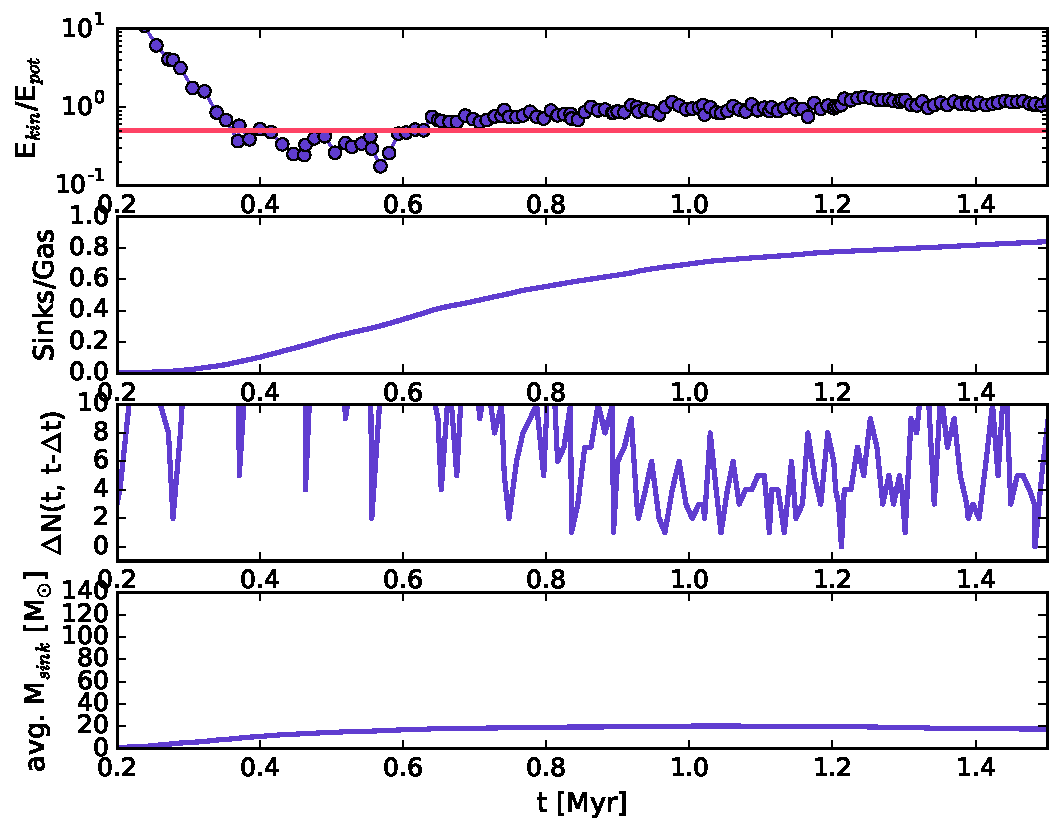
\includegraphics[width=0.9\textwidth]{Figures/cloud_plots/virial_noRTcloud}
 \captionsetup{justification=justified,singlelinecheck=false,width=\linewidth}
 \decoRule
 \caption[Reference run's virial analysis]{The virial analysis of the simulated cloud's star cluster in the reference run.
                                           In comparison with \figref{fig:Cluster_virial} we can see that at around 1.4 Myrs the reference run has already converted 80\% of all the present gas into sinks, while the RT--simulation has converted only 50\%.
                                           The overall sink formation rate also seems to be much higher.
                                           However, the average sink mass is lower in the reference run by almost a factor of 6.}
 \label{fig:Cluster_HDvirial}
\end{figure}
\FloatBarrier


%\newpage
% Conclusion ----------------------------------------------------------------------------------------
\section{Conclusion}
\label{sec:Conclusion}

% %TODO Conclusion chapter

In this thesis, radiation hydrodynamics simulations of sphere collapses and ultimately of a molecular cloud were presented.

After an introduction to the morphology of molecular clouds, the birth places of stars and star formation in general, the radiation hydrodynamics theory was construed.
The importance of the radiation's influence on star formation has been acknowledged by the astrophysics community since long and computer simulations gradually became efficient enough to numerically model radiation hydrodynamics directly.

To that end, in a subsequent chapter some numerical methods were described, which help implementing the radiation hydrodynamics theory into astrophysical simulation tools.
With the introduction of such a program, called RAMSES, which was used to perform the simulations in this thesis, the chapter was finished.
\\[6pt]
%
Here, in the last chapter, details to the different kinds of performed simulations were explained.

\begin{itemize}
  \item First, pure--hydrodynamics of core collapses were tested without radiation.
        Excessive fragmentation and a high number of low--mass sinks were typical outcomes of these simulations.
        However, this behavior was expected.
        They were intended to serve as reference for following tests to compare to and improve on.
  \item The second phase of runs involved and focused on the radiative transfer module of RAMSES, and in particular two parameters whose purpose were to optimize the numerical scheme.
        These parameters control the update of the reduced speed of light approximation and subcycling of the thermochemistry step, which calculates the effect of the (infrared) radiation onto matter.
        Although the computing times were almost doubled compared to the reference runs, an improvement concerning fragmentation could be observed.
        Around the sinks which act as radiation sources, the gas appeared much more diffuse due to the heat transfered by the infrared radiation.
        However, this effect is at most mid--ranged and fragmentation was not stopped in the outskirts of the spheres.
        The routines calculating the updates for the reduced speed of light approximation were deemed ineffective and not worth the computational resources.
  \item Subsequently, the disk stability of initially rotating singular isothermal sphere profiles was investigated with pure--hydrodynamics as well as radiative transfer simulations.
        Several variants of singular isothermal spheres were used as initial conditions with different masses and resolutions.
        Ulterior motives of these tests were to prepare to move to entire molecular clouds with a mass of the order of $\sim10^{4}$ M$_{\odot}$.
        The Toomre parameter analysis showed that disks are more stable when their gas is heated by the radiation.
        When the gas stays at 10 K, fragmentation causes disk instabilities.
  \item Finally, an entire molecular cloud with a mass of around $2.3\cdot10^{4}$ M$_{\odot}$ was simulated.
        Only a single photon group in the infrared spectrum was employed to investigate its isolated behavior.
        In the investigation of the radiation force from the most massive sink inside the cloud, it was concluded that even though the effect is slight, the force from radiation is able to withstand gravity to some degree.
        In comparison to the reference run of the same cloud, the sink particle number appeared to be considerably lower after $1.4$ Myrs, while the sink masses were much higher.
        It could be concluded that the infrared radiation effectively delays sink particle formation by heating the cloud's gas.
        The rise in gas temperature due to infrared radiation also must have affected the dynamics of the sink systems.
        Contrary to reference runs, several stable ternary systems were observed.
\end{itemize}

These simulations alone unfortunately are not enough to explain the low observed star formation efficiencies in our and nearby galaxies.
However, combined with higher energy photons in the ultraviolet spectrum from more massive stars, simulated star formation efficiencies could already approach the observed numbers.
Nevertheless, radiation definitely improves our understanding of star formation.
In the future, radiative transfer routines will definitely be improved through either utilization of GPUs or improvements in numerical schemes such as faster implicit time stepping methods.
It might even not be long until simulations involving radiation hydrodynamics and magnetohydrodynamics can be efficiently performed to gain even deeper understanding in star formation.
